% This is a sample LaTeX input file.  (Version of 11 April 1994.)
%
% A '%' character causes TeX to ignore all remaining text on the line,
% and is used for comments like this one.

\documentclass[11pt]{article}      % Specifies the document class
\usepackage{amsfonts,amssymb,amsmath}
\topmargin-0.2in
\textheight9.0in
\oddsidemargin-0.2in
\evensidemargin-0.2in
\textwidth6.5in

\usepackage{graphicx} % Required for inserting images
\usepackage{booktabs}
\usepackage{subcaption}
\usepackage{xcolor}  

\usepackage{listings}
\lstset{
	basicstyle=\footnotesize\ttfamily,
	columns=flexible,
	breaklines=true,
	commentstyle=\color{red},
	keywordstyle=\color{black}\bfseries}

\newcommand{\mZ}{\mathbb Z}
\newcommand{\mR}{\mathbb R}
\newcommand{\mC}{\mathbb C}
\newcommand{\mQ}{\mathbb Q}
\newcommand{\ep}{\epsilon}
\begin{document}             % End of preamble and beginning of text.

%\thispagestyle{empty}
\begin{center}
{\bf\large HW4(FEA): Appiah Francis}\\
\vspace{0.05in}
\end{center}
%--- coding
\begin{enumerate}
\item[Case 1: ] RB space $V_m = \text{span}\{U_h(\mu_j), j =1,\ldots,m\}$, with $L_1$ error indicator
\begin{figure}[htbp]
	\centering
	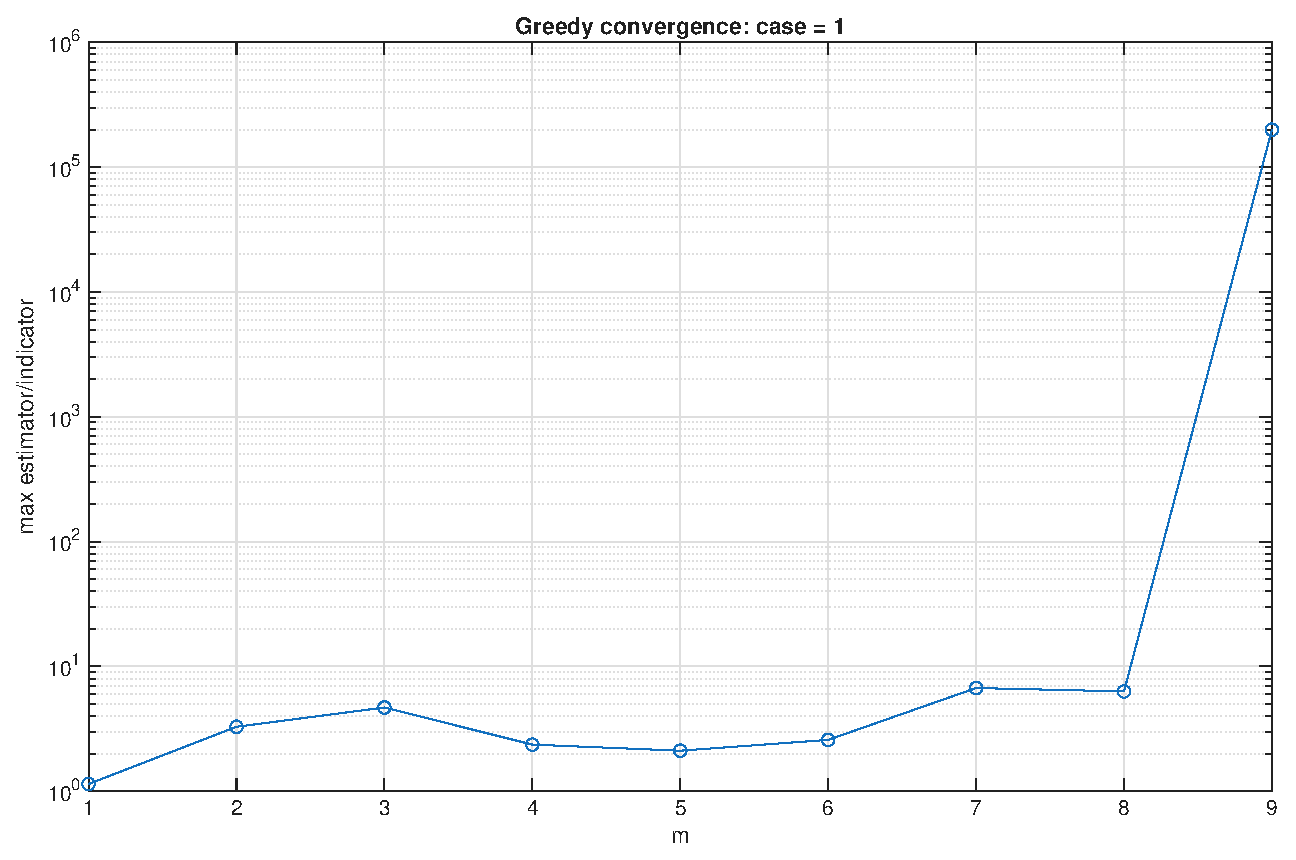
\includegraphics[width=0.5\textwidth]{img/GC_case1_basis1_err1.eps}
    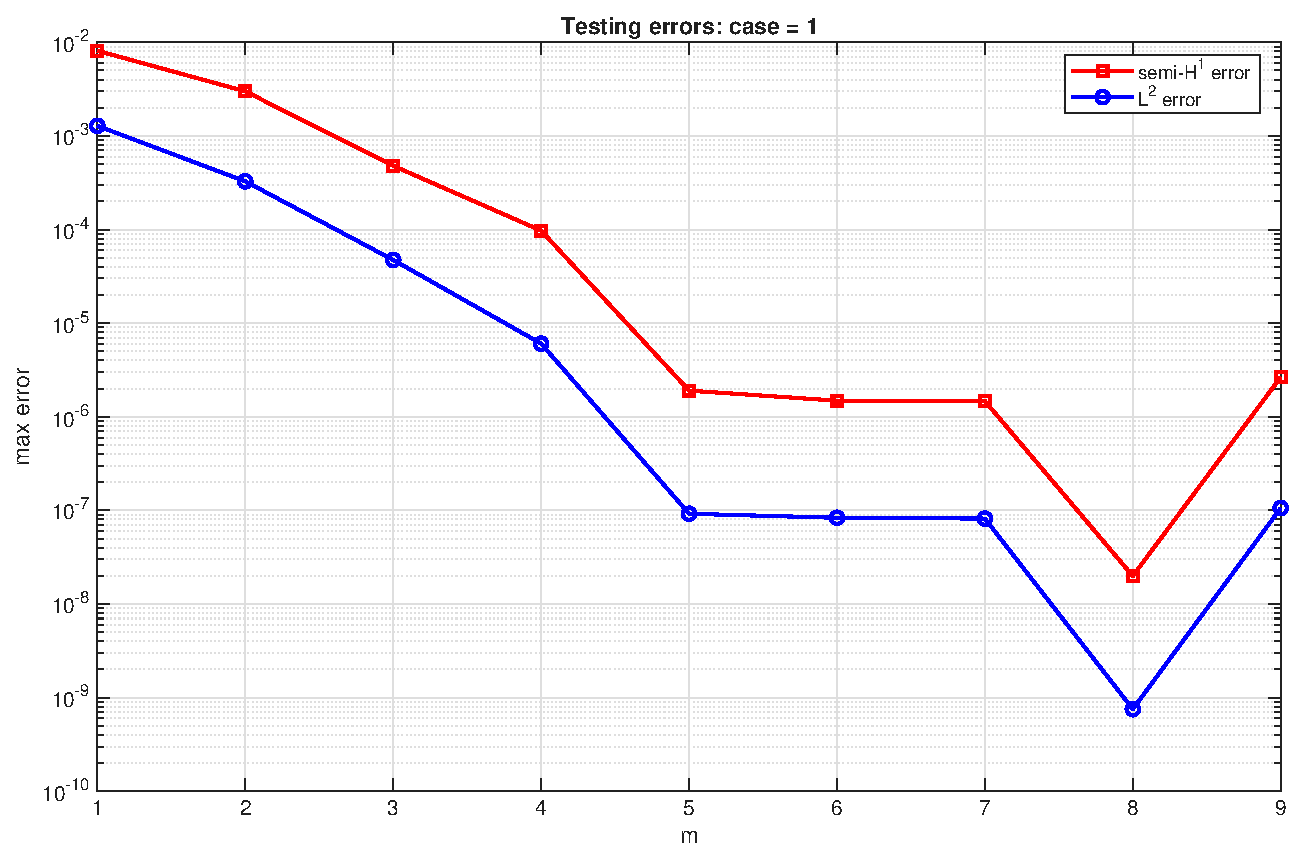
\includegraphics[width=0.5\textwidth]{img/TE_case1_basis1_err1.eps}
    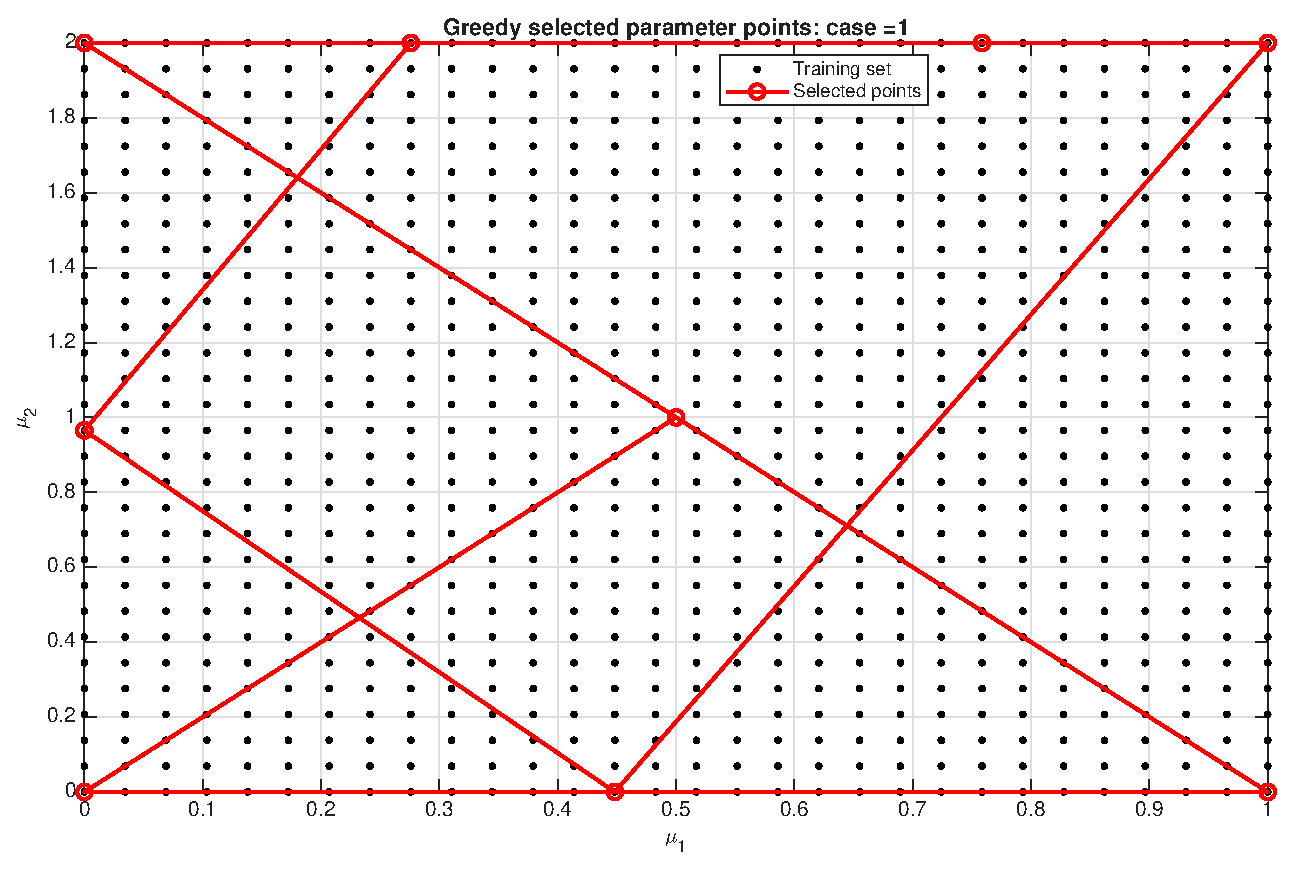
\includegraphics[width=0.5\textwidth]{img/GSP_case1_basis1_err1.eps}
%	
\includegraphics[width=0.29\textwidth]{img/solplot_N80_k15_k29.eps}
%	\caption{Graph of FEM and Exact solution When $x_k =0.5$ is a node}
%	\label{fig:N1}
\end{figure}
\clearpage
\item[Case 1: ] RB space $V_m = \text{span}\{U_h(\mu_j), j =1,\ldots,m\}$, with residual error estimator
\begin{figure}[htbp]
	\centering
	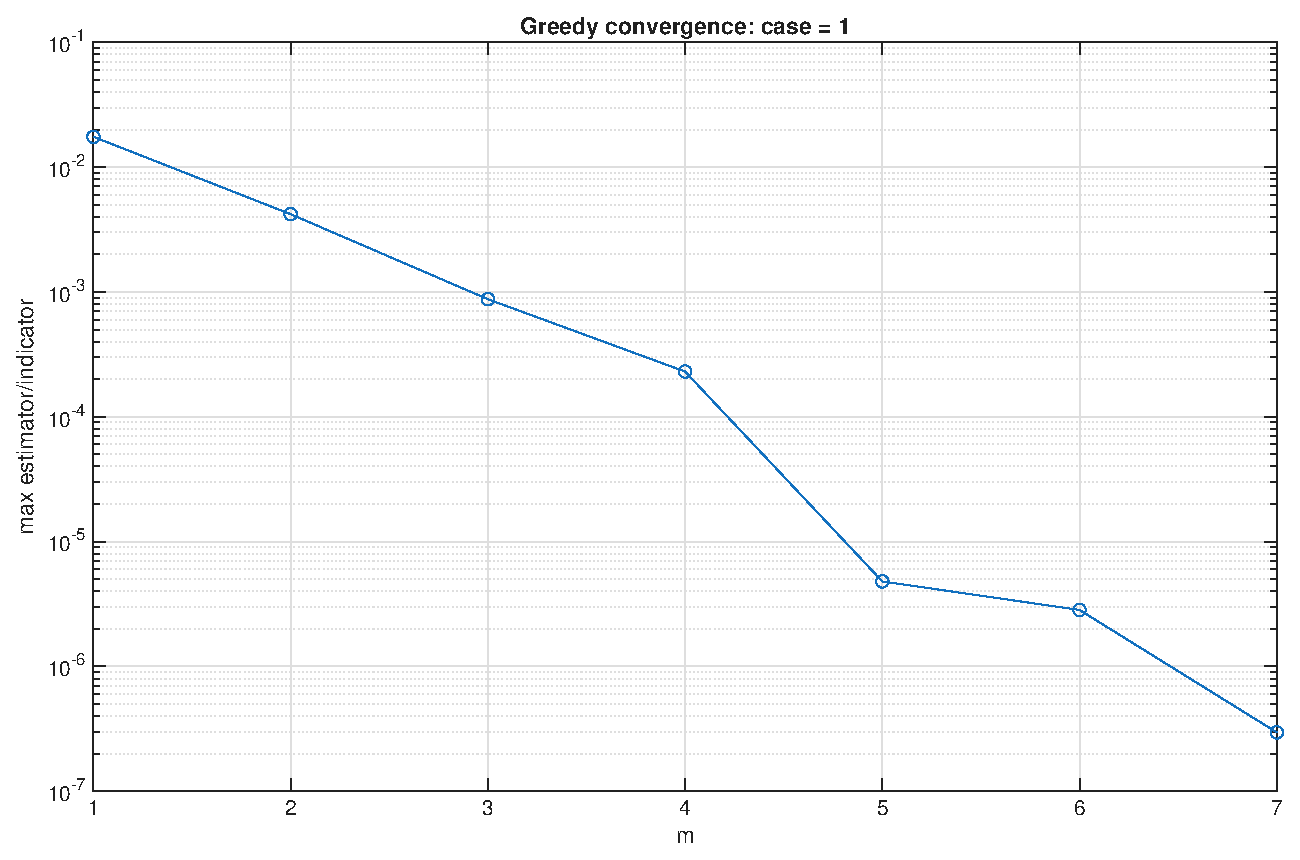
\includegraphics[width=0.5\textwidth]{img/GC_case1_basis1_err2.eps}
	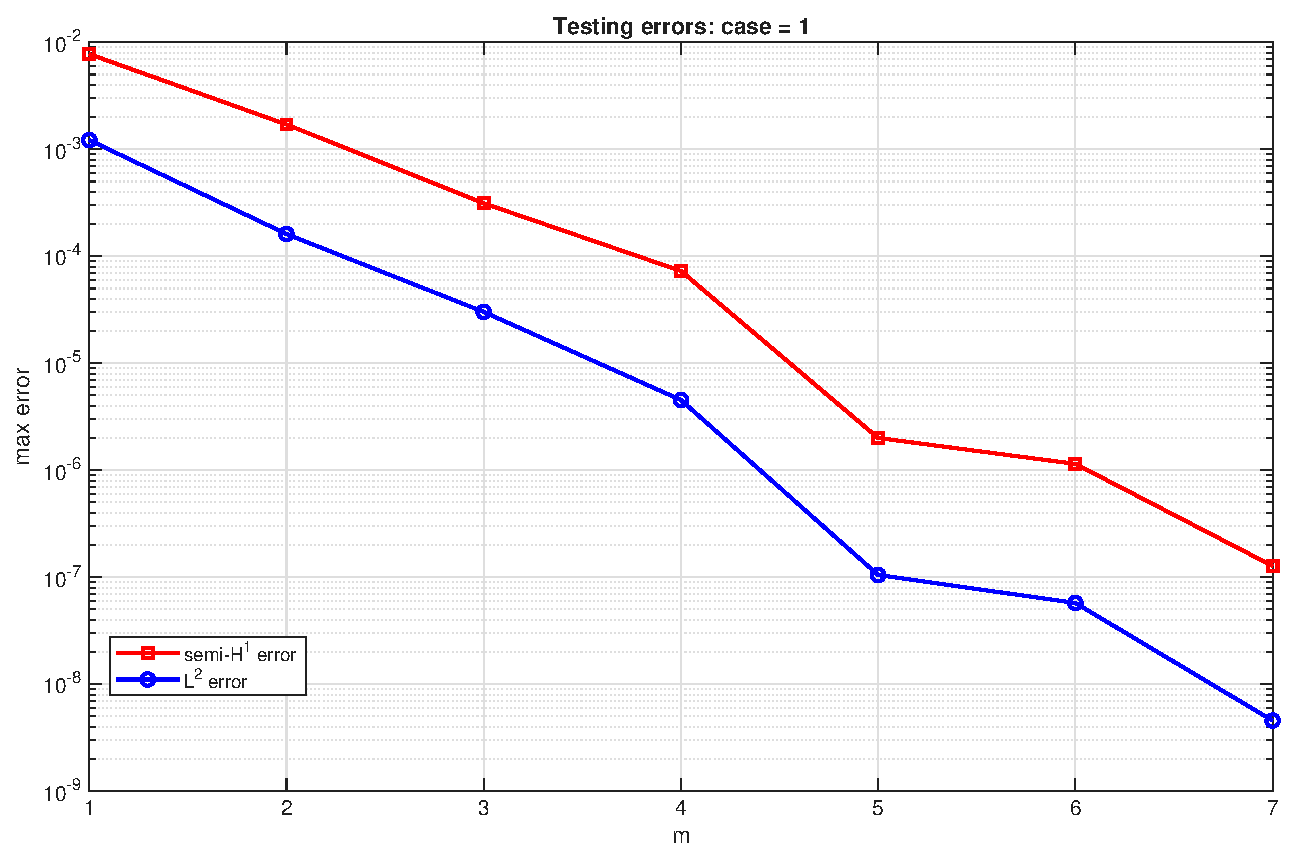
\includegraphics[width=0.5\textwidth]{img/TE_case1_basis1_err2.eps}
	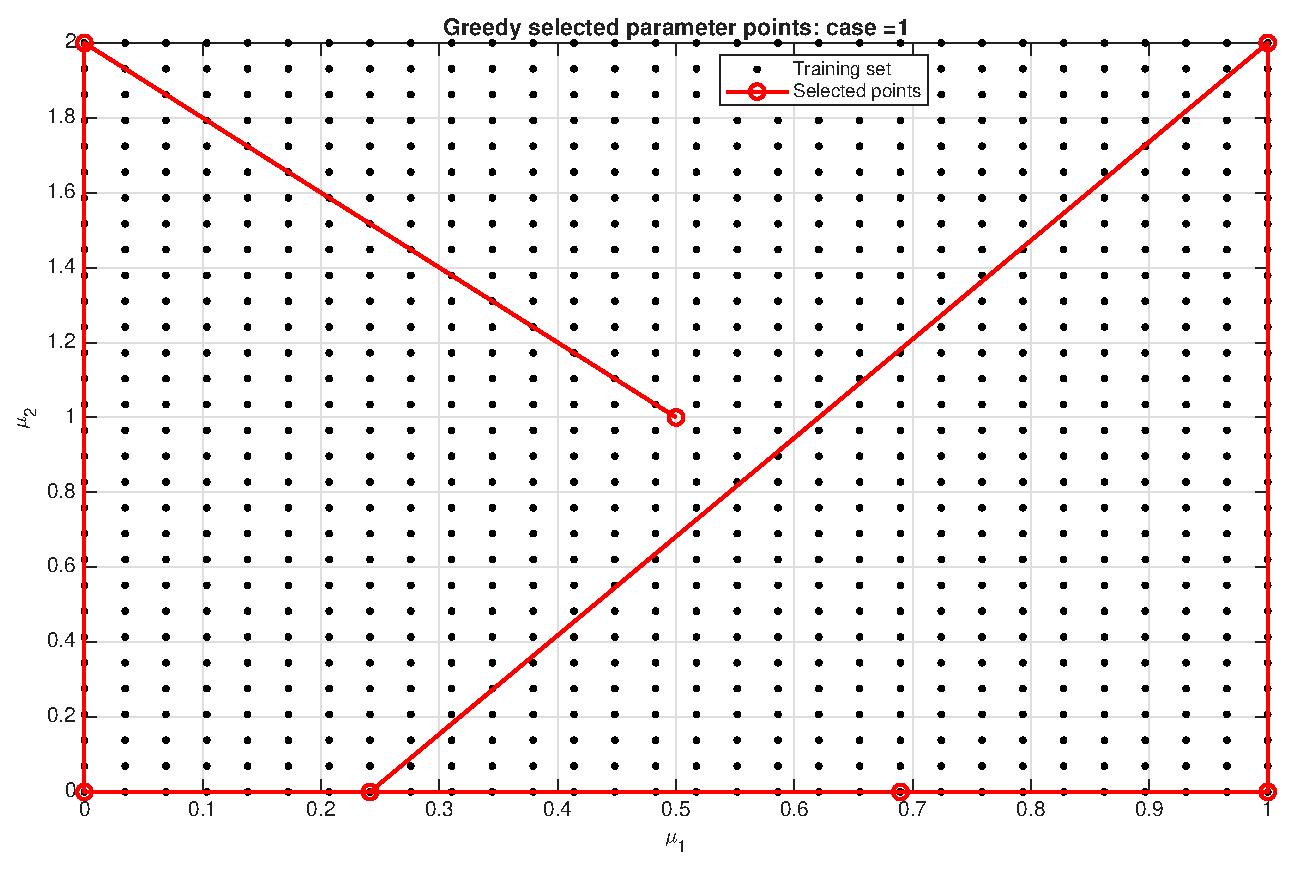
\includegraphics[width=0.5\textwidth]{img/GSP_case1_basis1_err2.eps}
	%	
\includegraphics[width=0.29\textwidth]{img/solplot_N80_k15_k29.eps}
	%	\caption{Graph of FEM and Exact solution When $x_k =0.5$ is a node}
	%	\label{fig:N1}
\end{figure}
\clearpage
\item[Case 1: ] QR factorization, with $L_1$ error indicator
\begin{figure}[htbp]
	\centering
	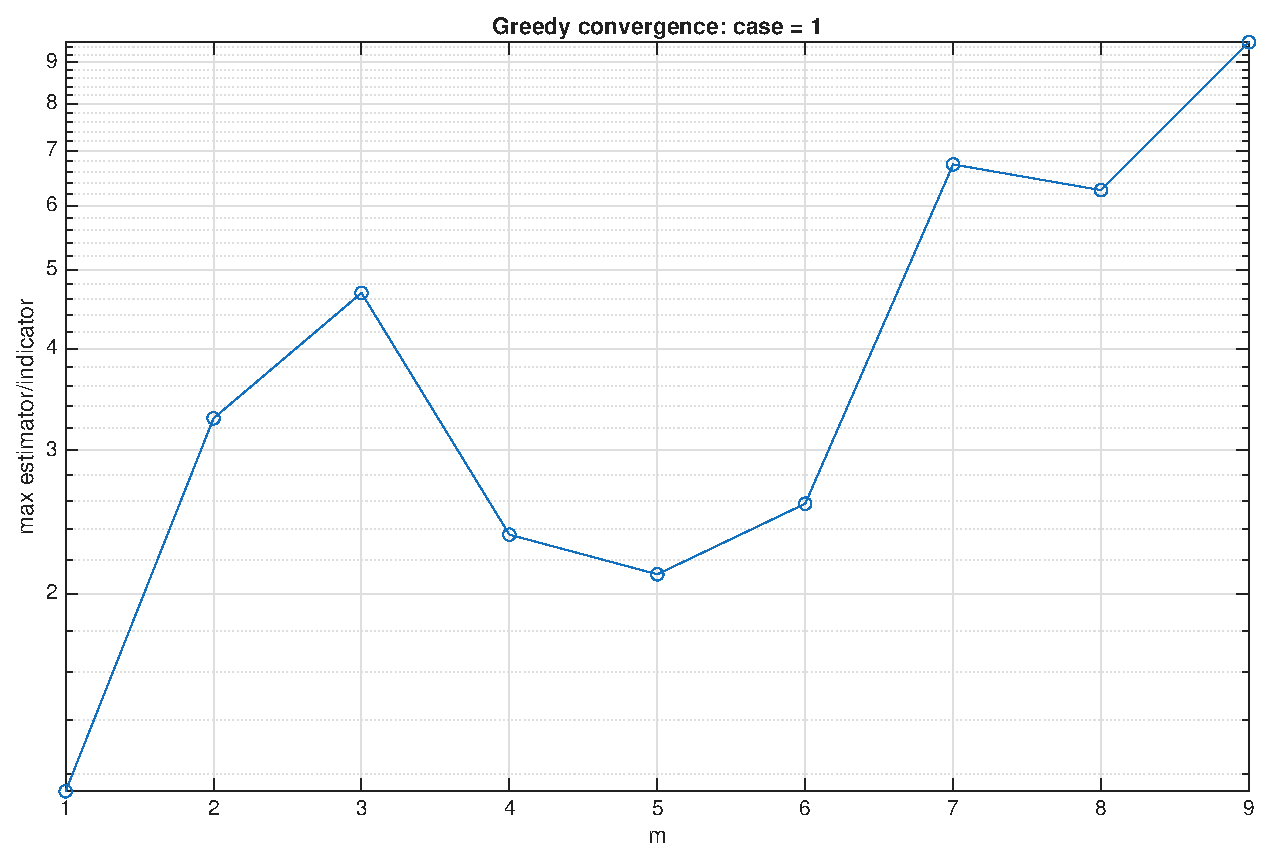
\includegraphics[width=0.5\textwidth]{img/GC_case1_basis2_err1.eps}
	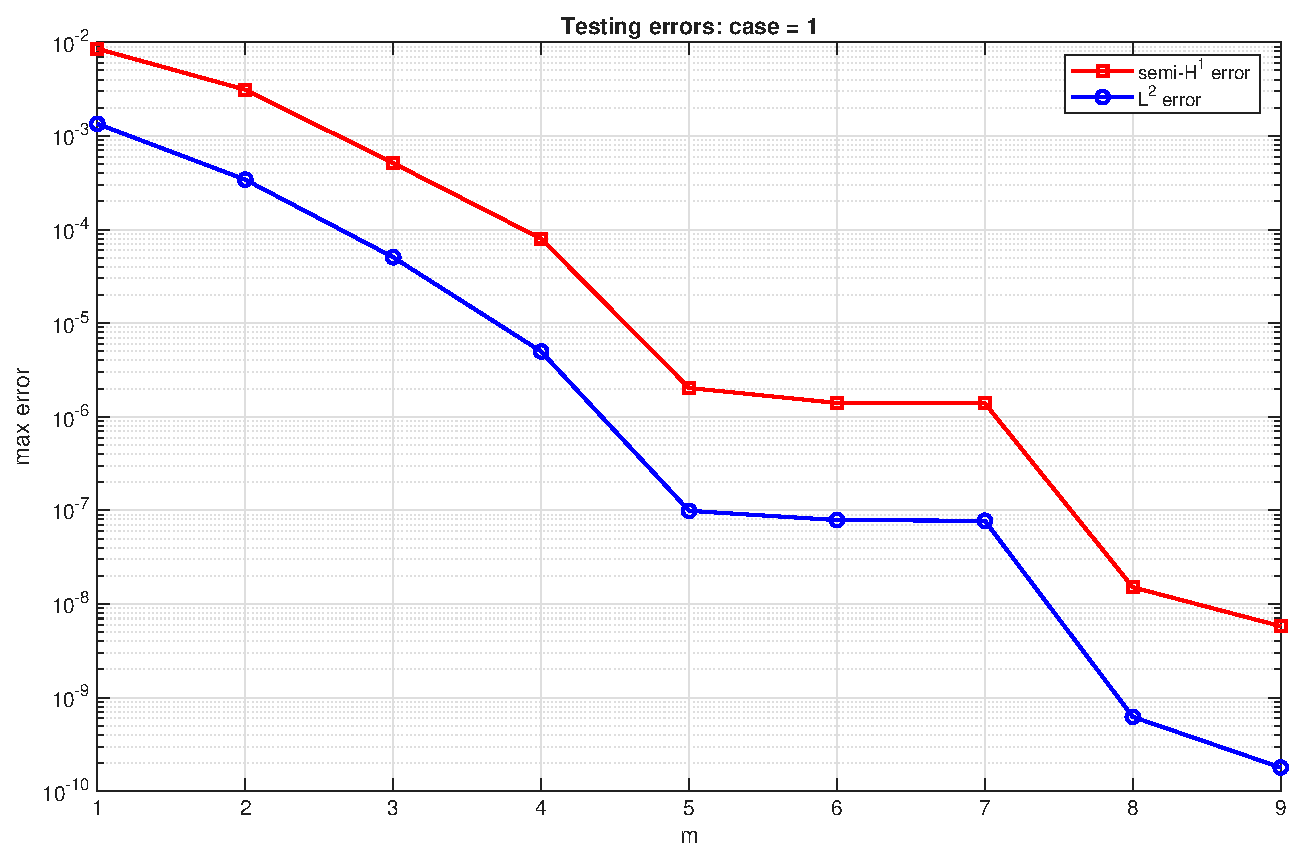
\includegraphics[width=0.5\textwidth]{img/TE_case1_basis2_err1.eps}
	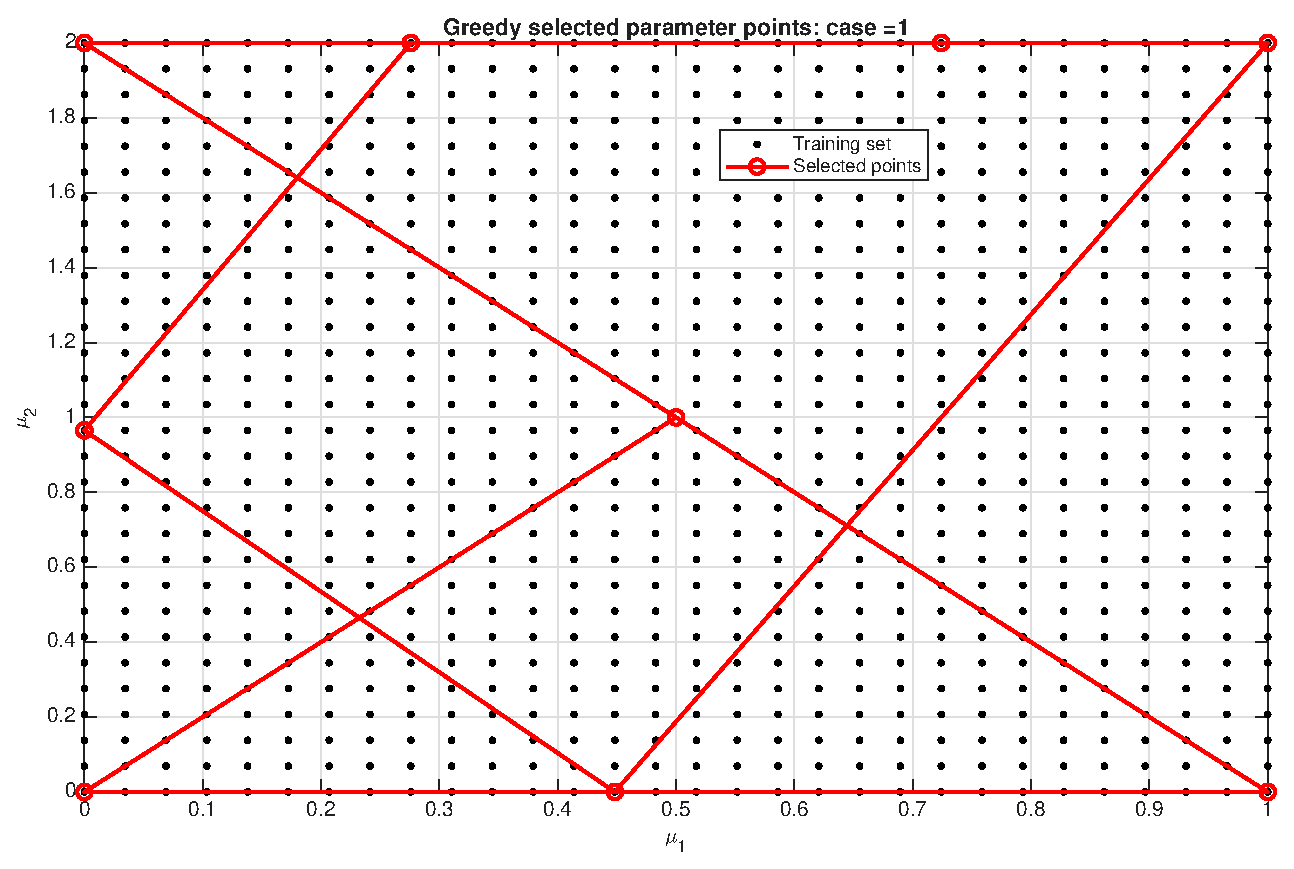
\includegraphics[width=0.5\textwidth]{img/GSP_case1_basis2_err1.eps}
	%	
\includegraphics[width=0.29\textwidth]{img/solplot_N80_k15_k29.eps}
	%	\caption{Graph of FEM and Exact solution When $x_k =0.5$ is a node}
	%	\label{fig:N1}
\end{figure}
\clearpage
\item[Case 1: ] QR factorization, with residual error estimator
\begin{figure}[htbp]
	\centering
	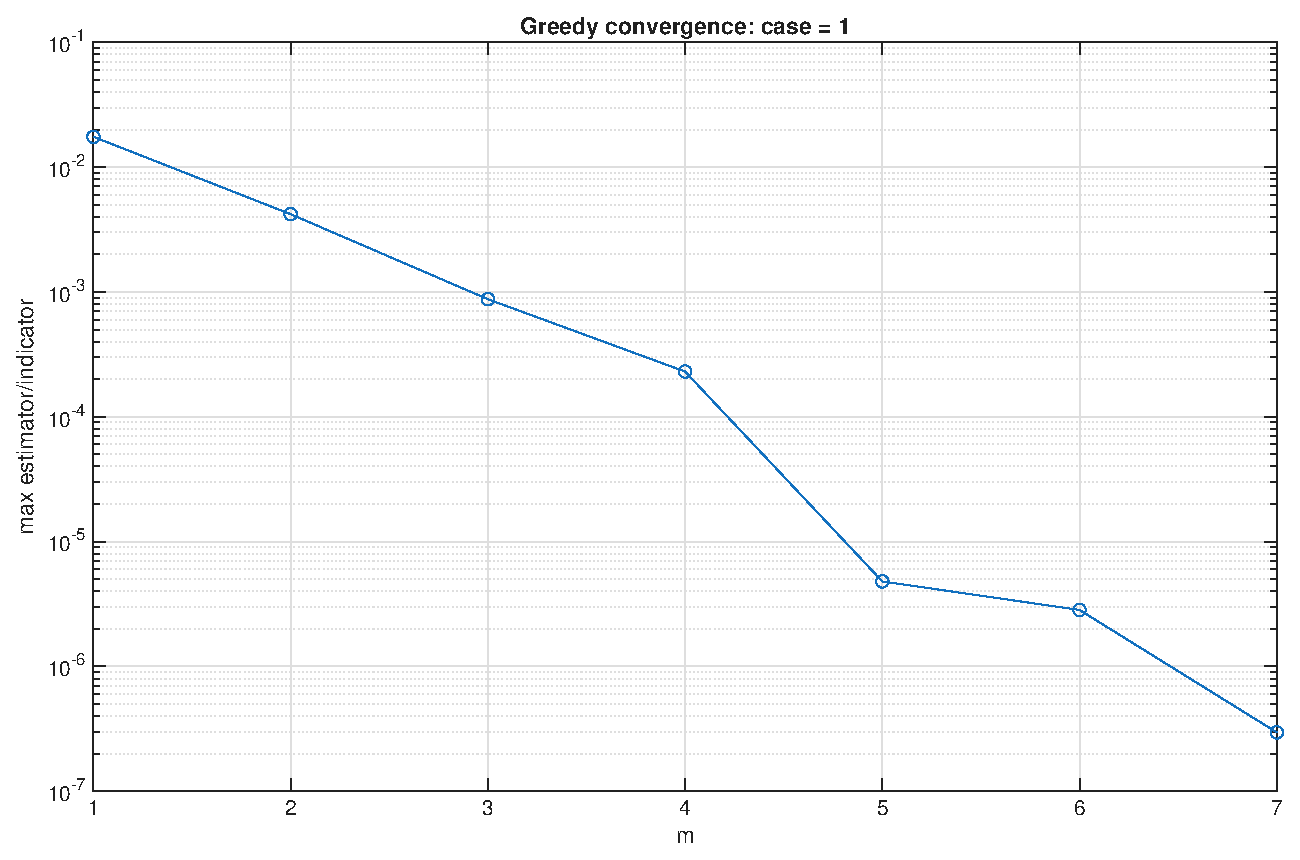
\includegraphics[width=0.5\textwidth]{img/GC_case1_basis2_err2.eps}
	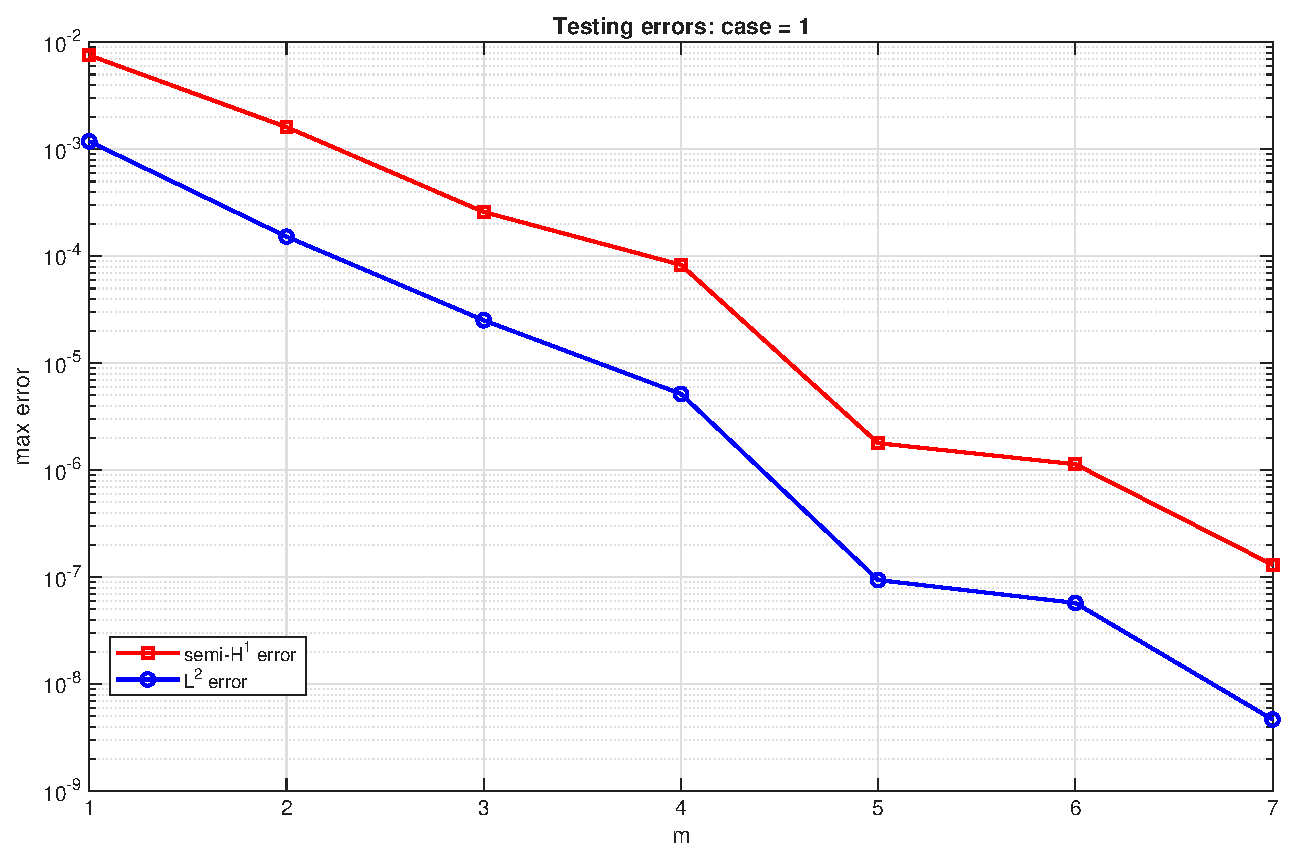
\includegraphics[width=0.5\textwidth]{img/TE_case1_basis2_err2.eps}
	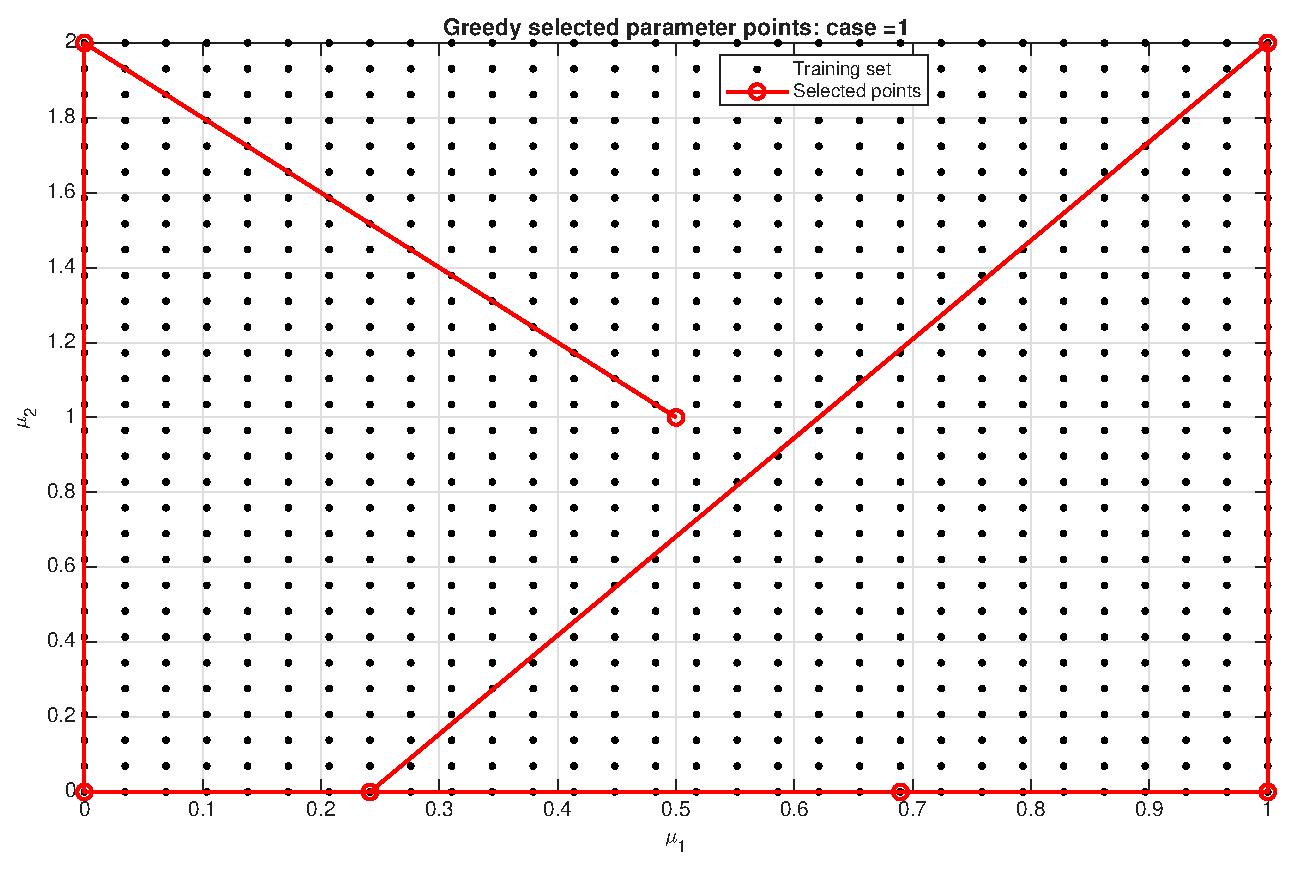
\includegraphics[width=0.5\textwidth]{img/GSP_case1_basis2_err2.eps}
	%	
\includegraphics[width=0.29\textwidth]{img/solplot_N80_k15_k29.eps}
	%	\caption{Graph of FEM and Exact solution When $x_k =0.5$ is a node}
	%	\label{fig:N1}
\end{figure}
\clearpage
\item[Case 2: ] RB space $V_m = \text{span}\{U_h(\mu_j), j =1,\ldots,m\}$, with $L_1$ error indicator
\begin{figure}[htbp]
	\centering
	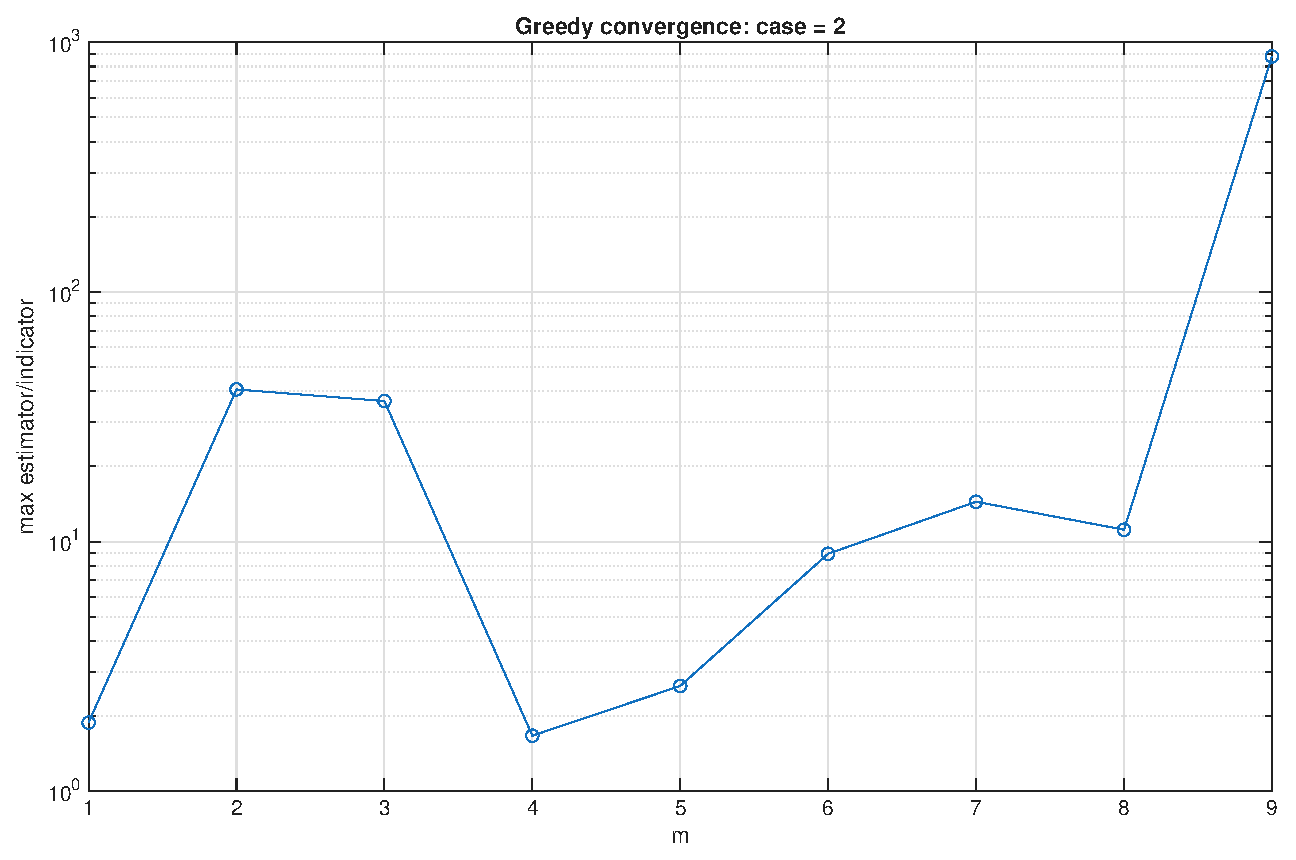
\includegraphics[width=0.5\textwidth]{img/GC_case2_basis1_err1.eps}
	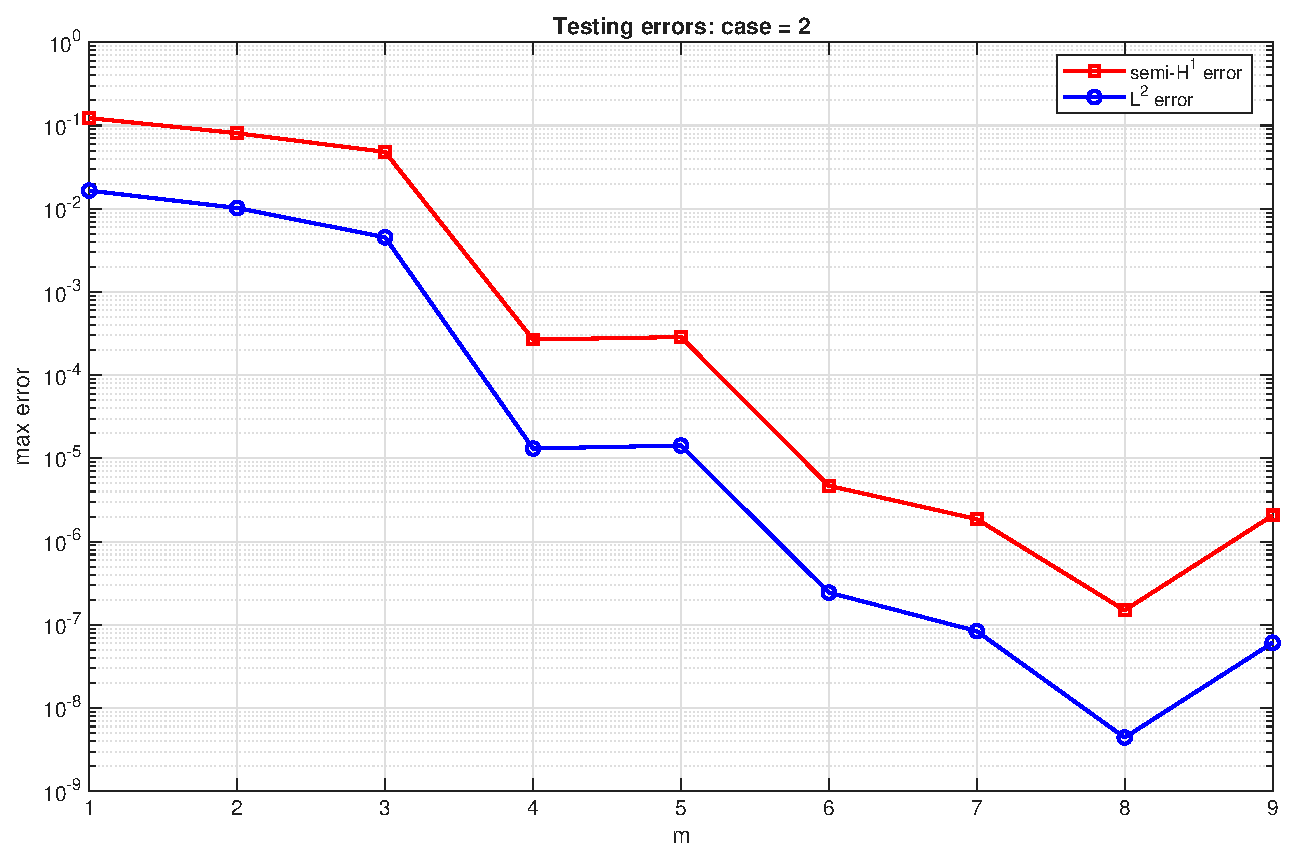
\includegraphics[width=0.5\textwidth]{img/TE_case2_basis1_err1.eps}
	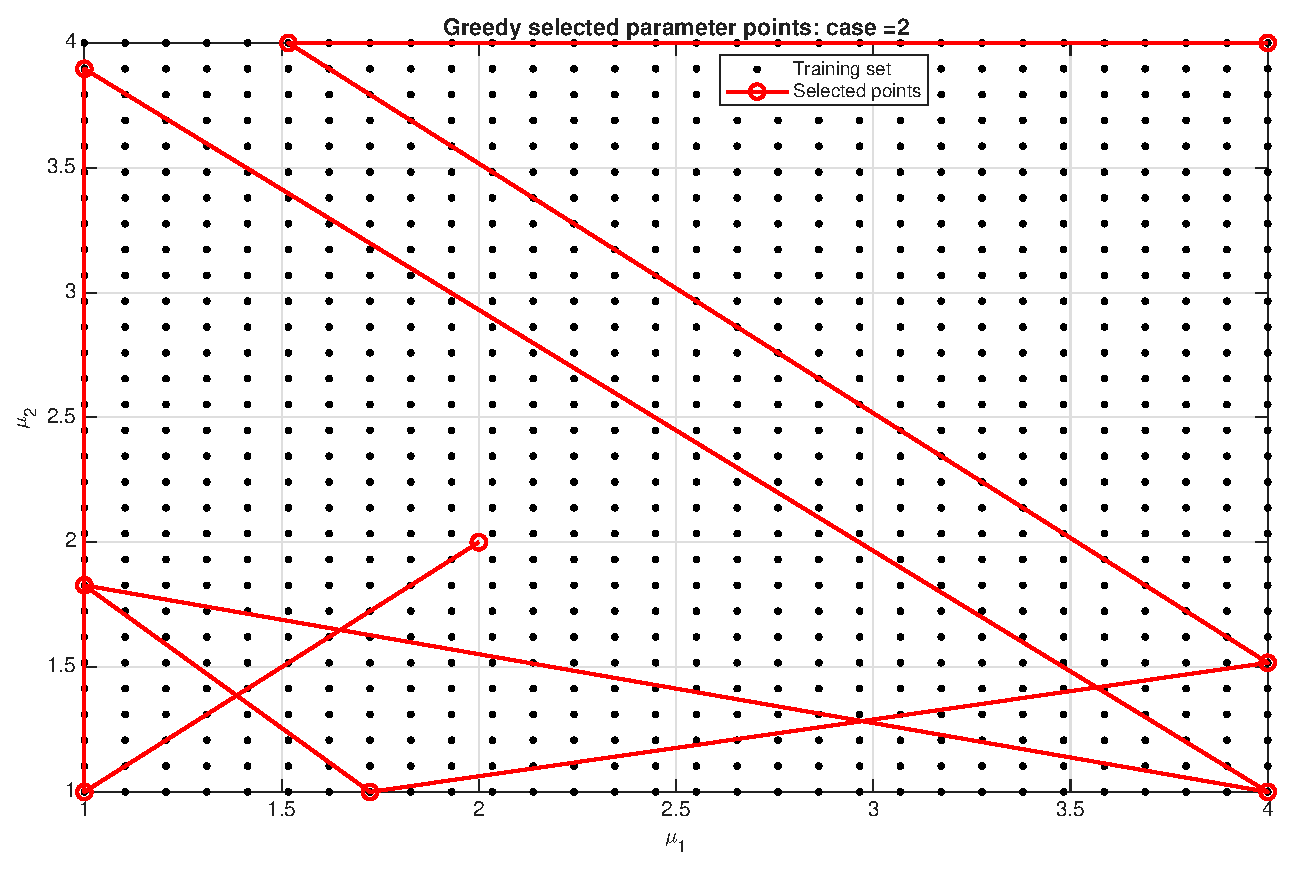
\includegraphics[width=0.5\textwidth]{img/GSP_case2_basis1_err1.eps}
	%	
\includegraphics[width=0.29\textwidth]{img/solplot_N80_k15_k29.eps}
	%	\caption{Graph of FEM and Exact solution When $x_k =0.5$ is a node}
	%	\label{fig:N1}
\end{figure}
\clearpage
\item[Case 2: ] RB space $V_m = \text{span}\{U_h(\mu_j), j =1,\ldots,m\}$, with residual error estimator
\begin{figure}[htbp]
	\centering
	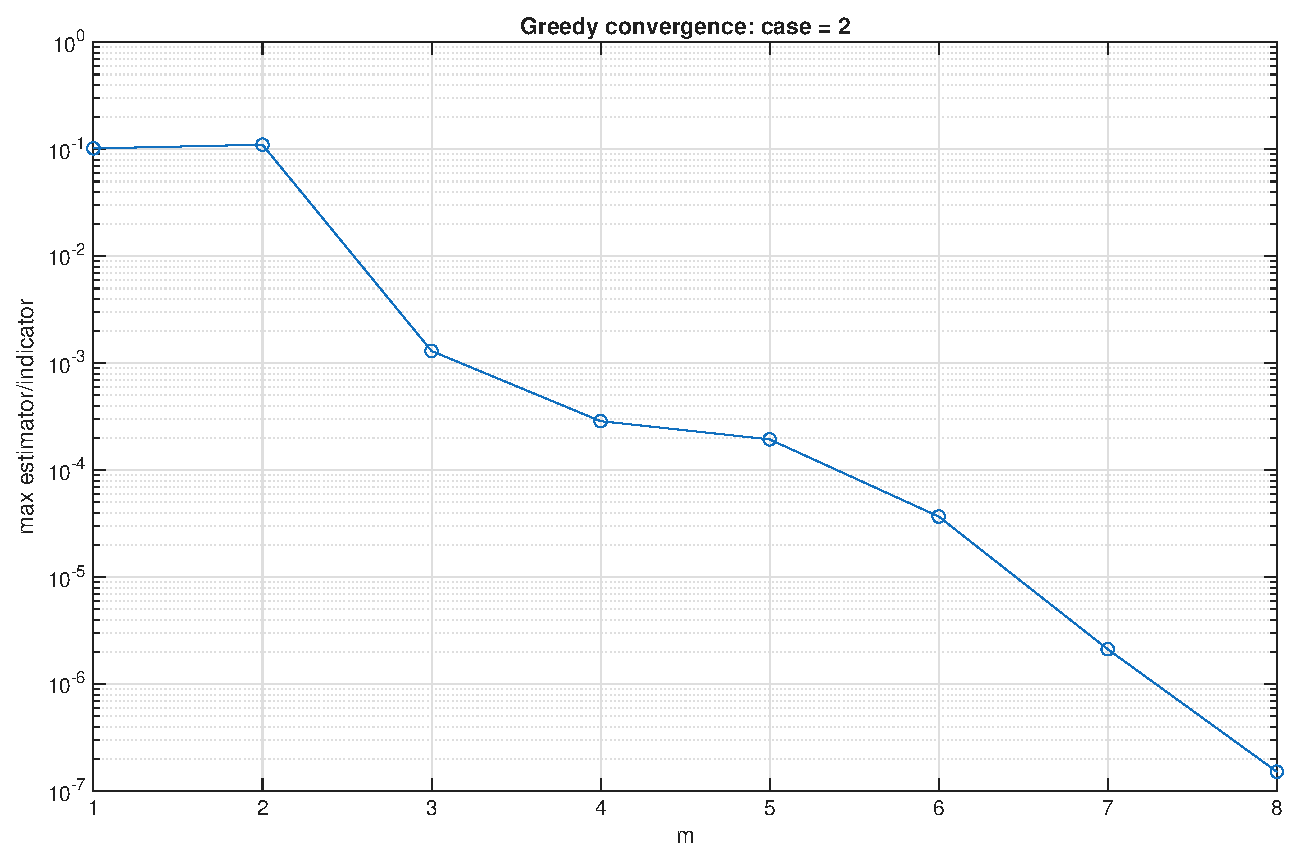
\includegraphics[width=0.5\textwidth]{img/GC_case2_basis1_err2.eps}
	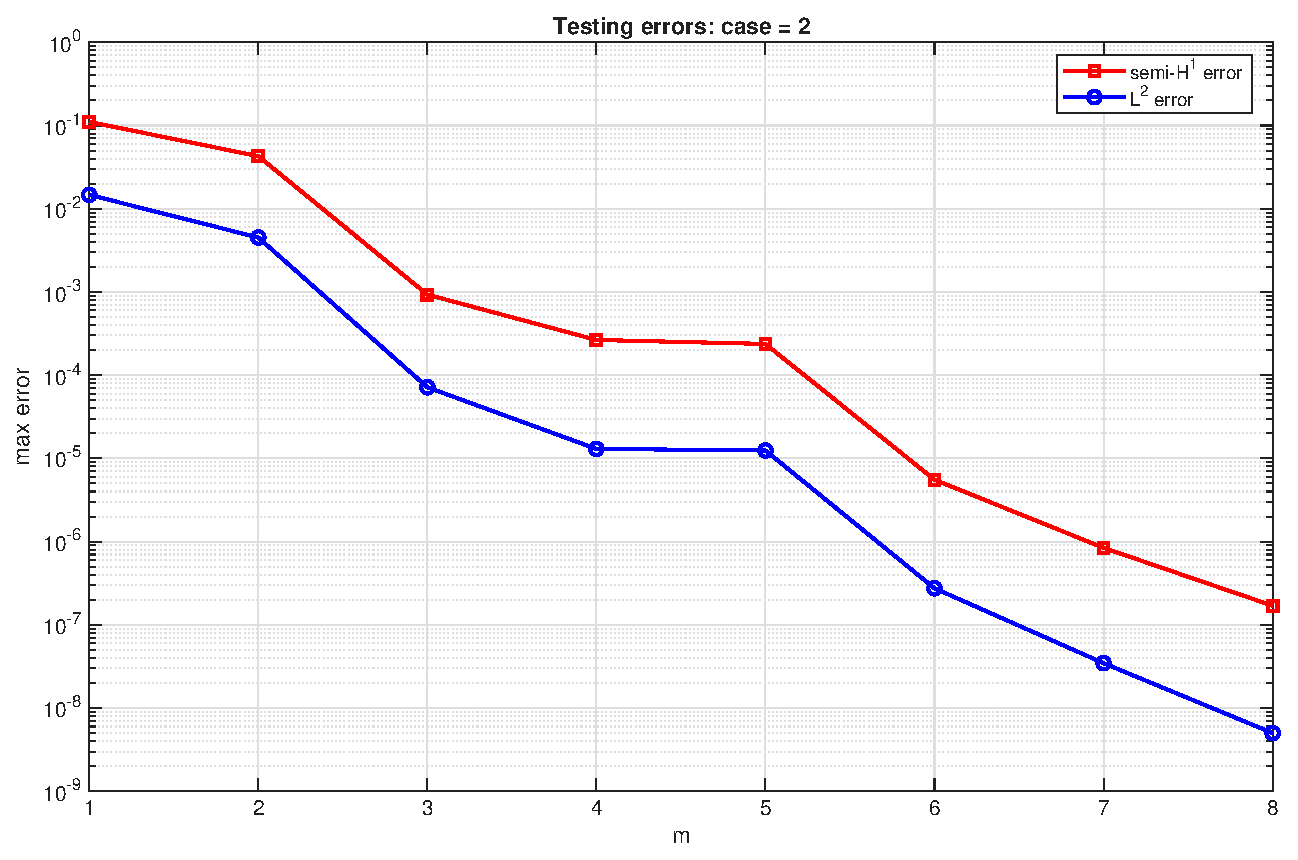
\includegraphics[width=0.5\textwidth]{img/TE_case2_basis1_err2.eps}
	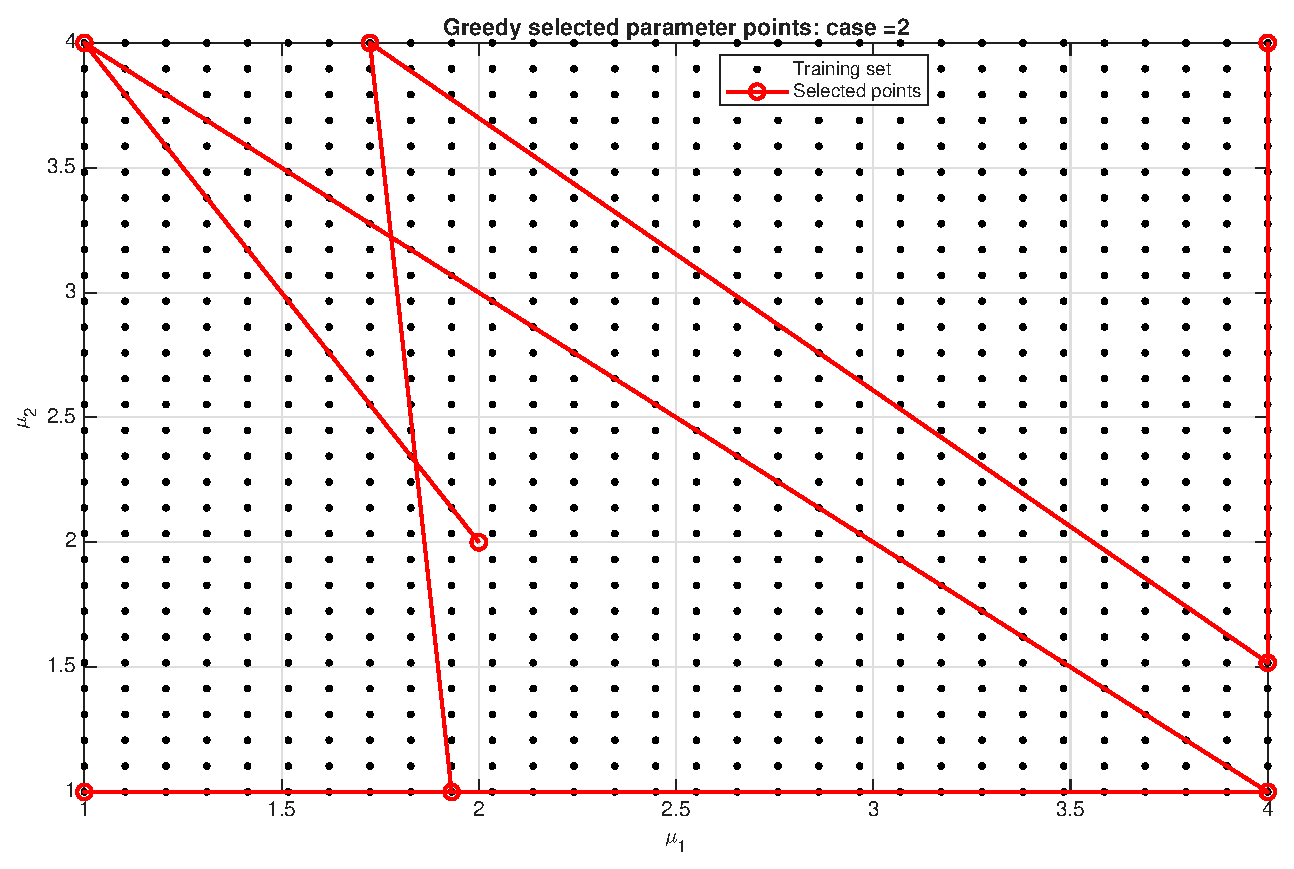
\includegraphics[width=0.5\textwidth]{img/GSP_case2_basis1_err2.eps}
	%	
\includegraphics[width=0.29\textwidth]{img/solplot_N80_k15_k29.eps}
	%	\caption{Graph of FEM and Exact solution When $x_k =0.5$ is a node}
	%	\label{fig:N1}
\end{figure}
\clearpage
\item[Case 2: ] QR factorization, with $L_1$ error indicator
\begin{figure}[htbp]
	\centering
	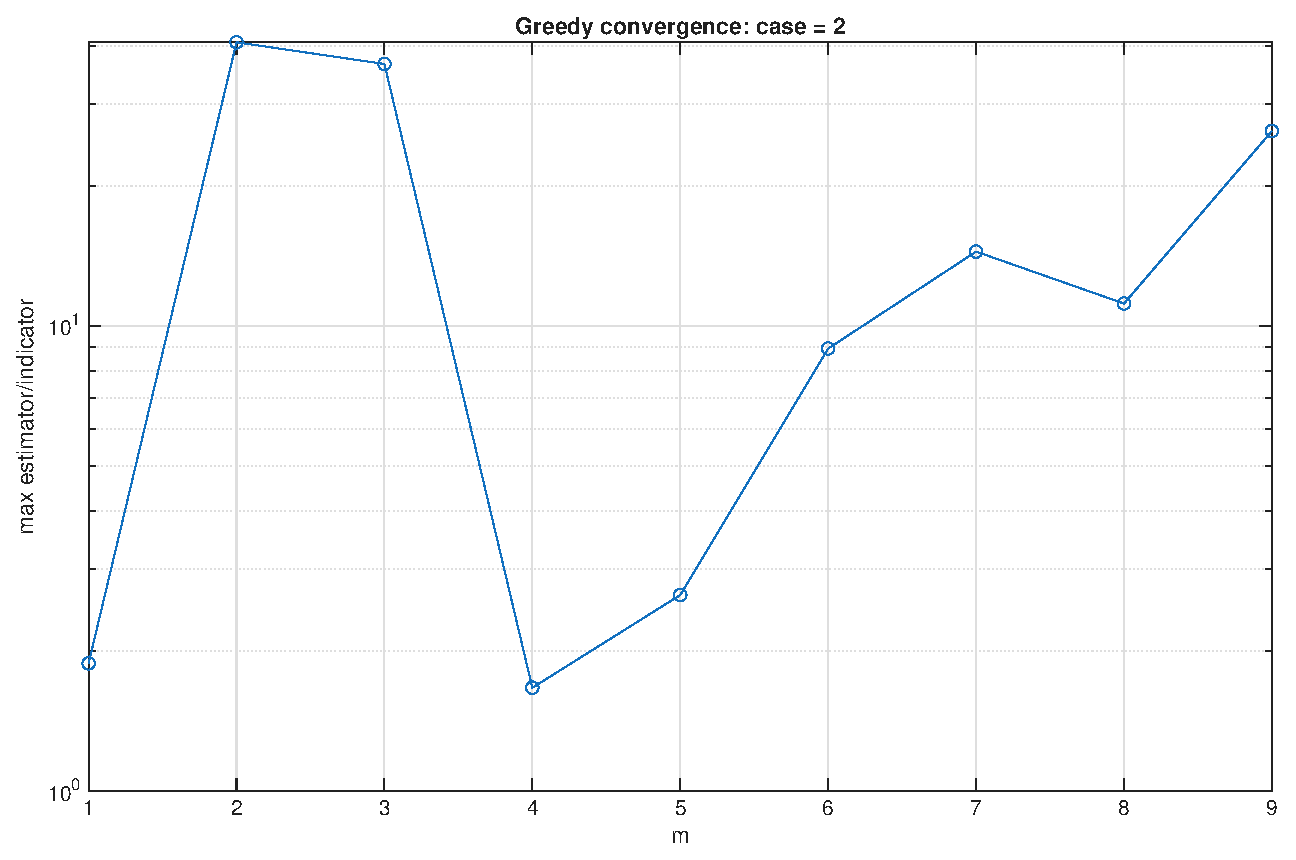
\includegraphics[width=0.5\textwidth]{img/GC_case2_basis2_err1.eps}
	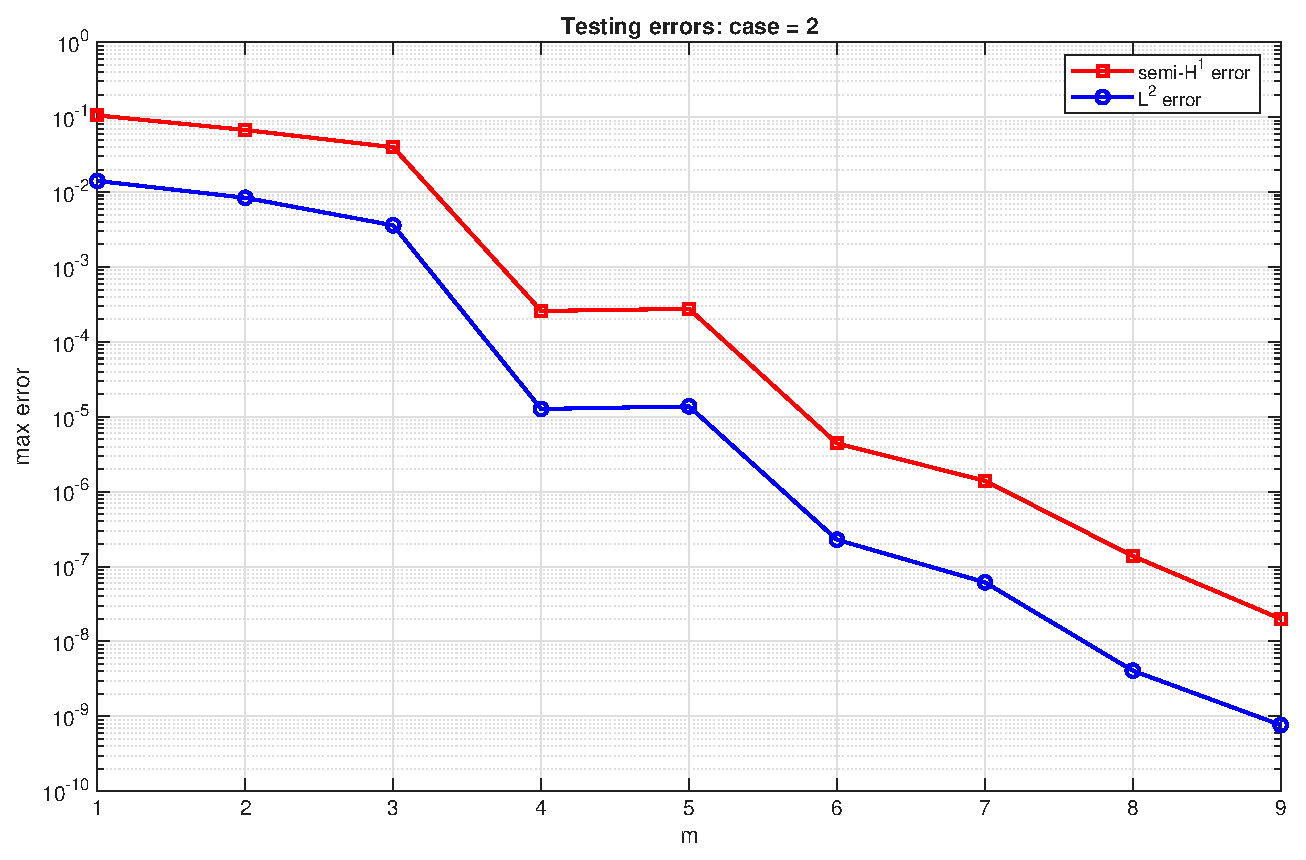
\includegraphics[width=0.5\textwidth]{img/TE_case2_basis2_err1.eps}
	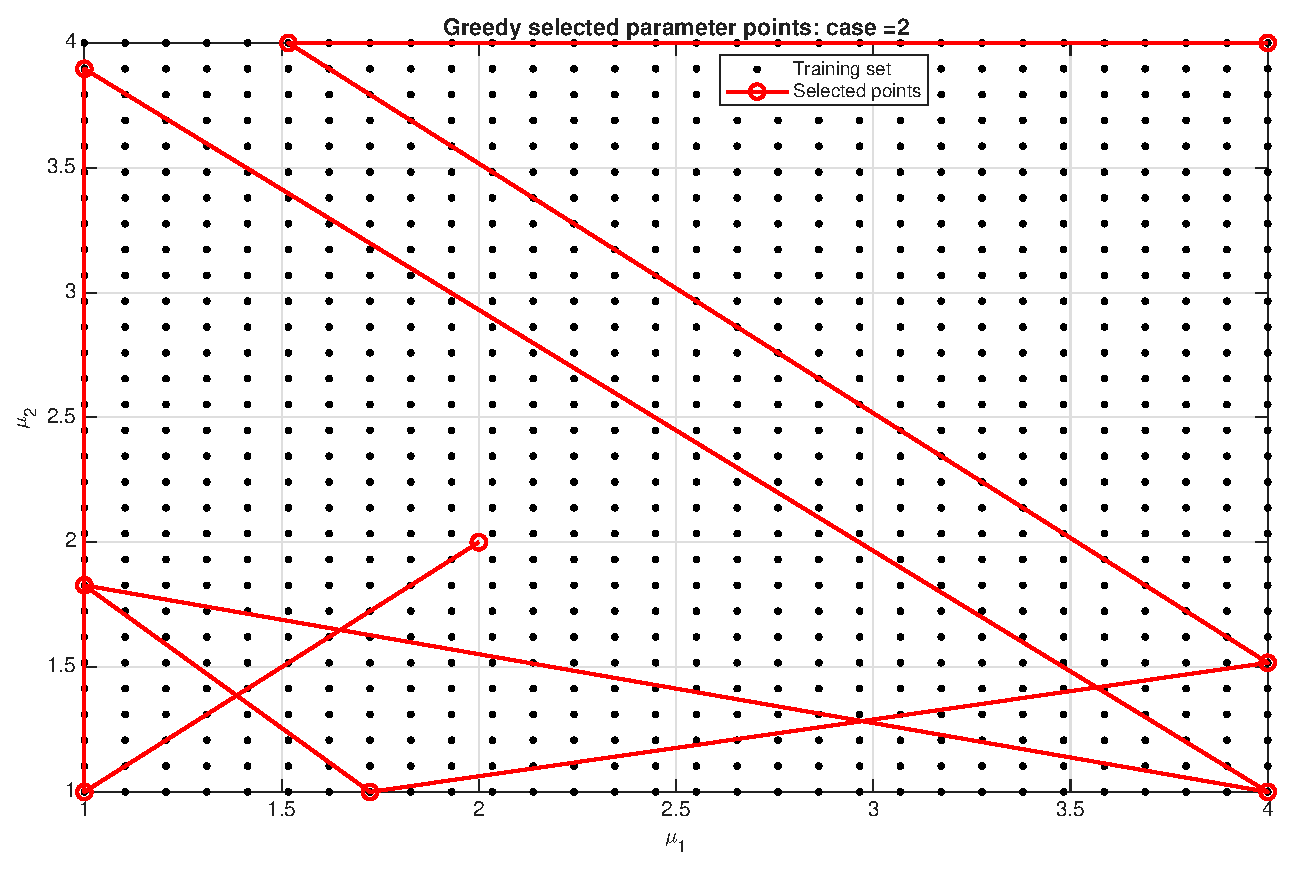
\includegraphics[width=0.5\textwidth]{img/GSP_case2_basis2_err1.eps}
	%	
\includegraphics[width=0.29\textwidth]{img/solplot_N80_k15_k29.eps}
	%	\caption{Graph of FEM and Exact solution When $x_k =0.5$ is a node}
	%	\label{fig:N1}
\end{figure}
\clearpage
\item[Case 2: ] QR factorization, with residual error estimator
\begin{figure}[htbp]
	\centering
	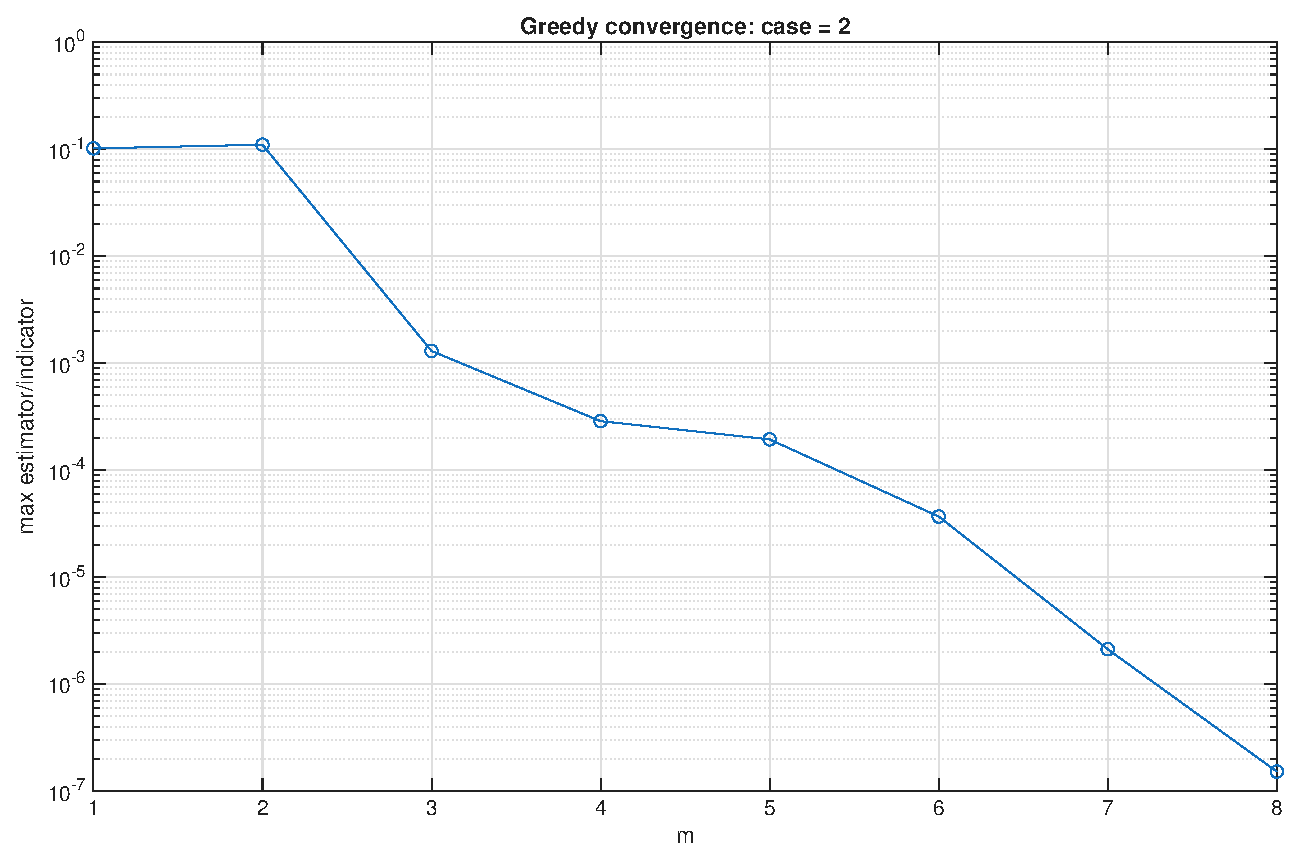
\includegraphics[width=0.5\textwidth]{img/GC_case2_basis2_err2.eps}
	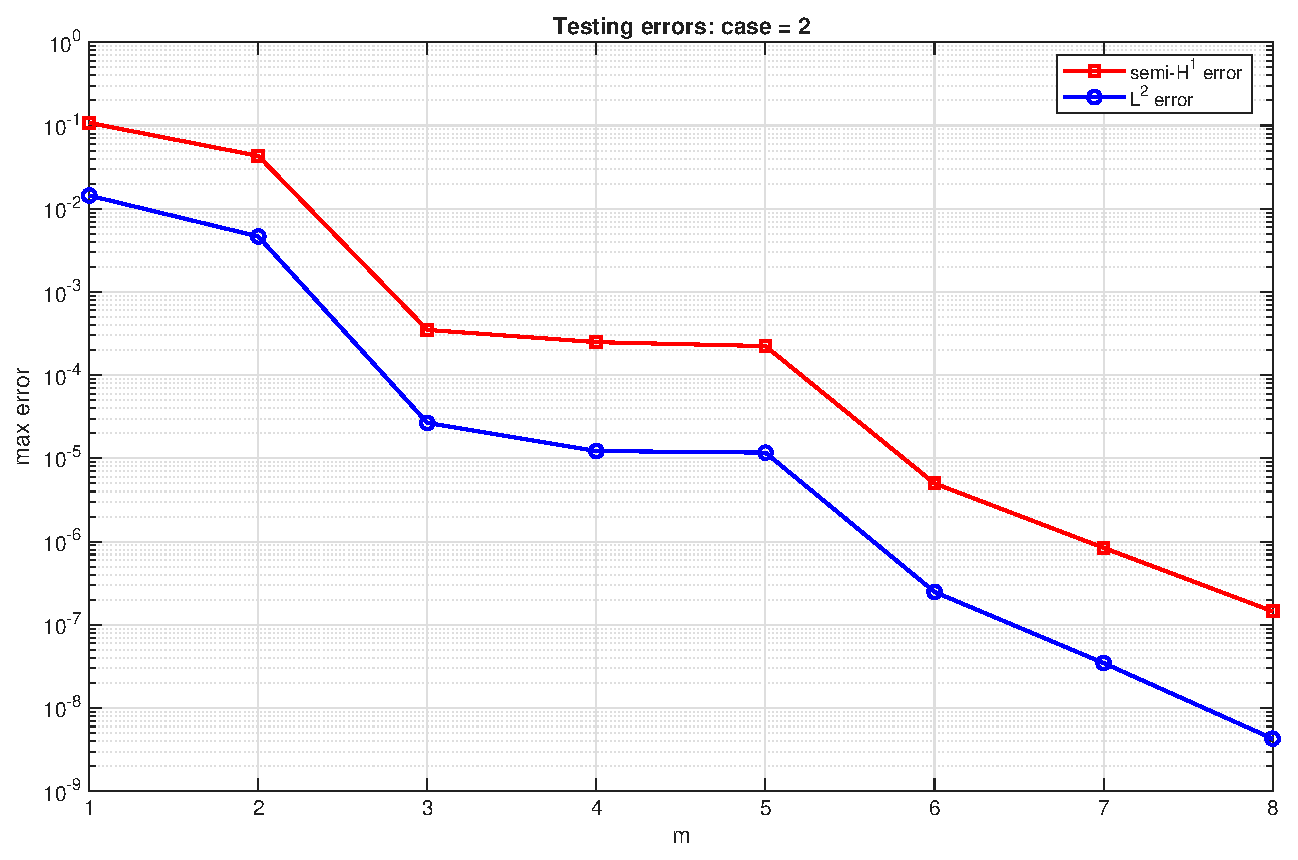
\includegraphics[width=0.5\textwidth]{img/TE_case2_basis2_err2.eps}
	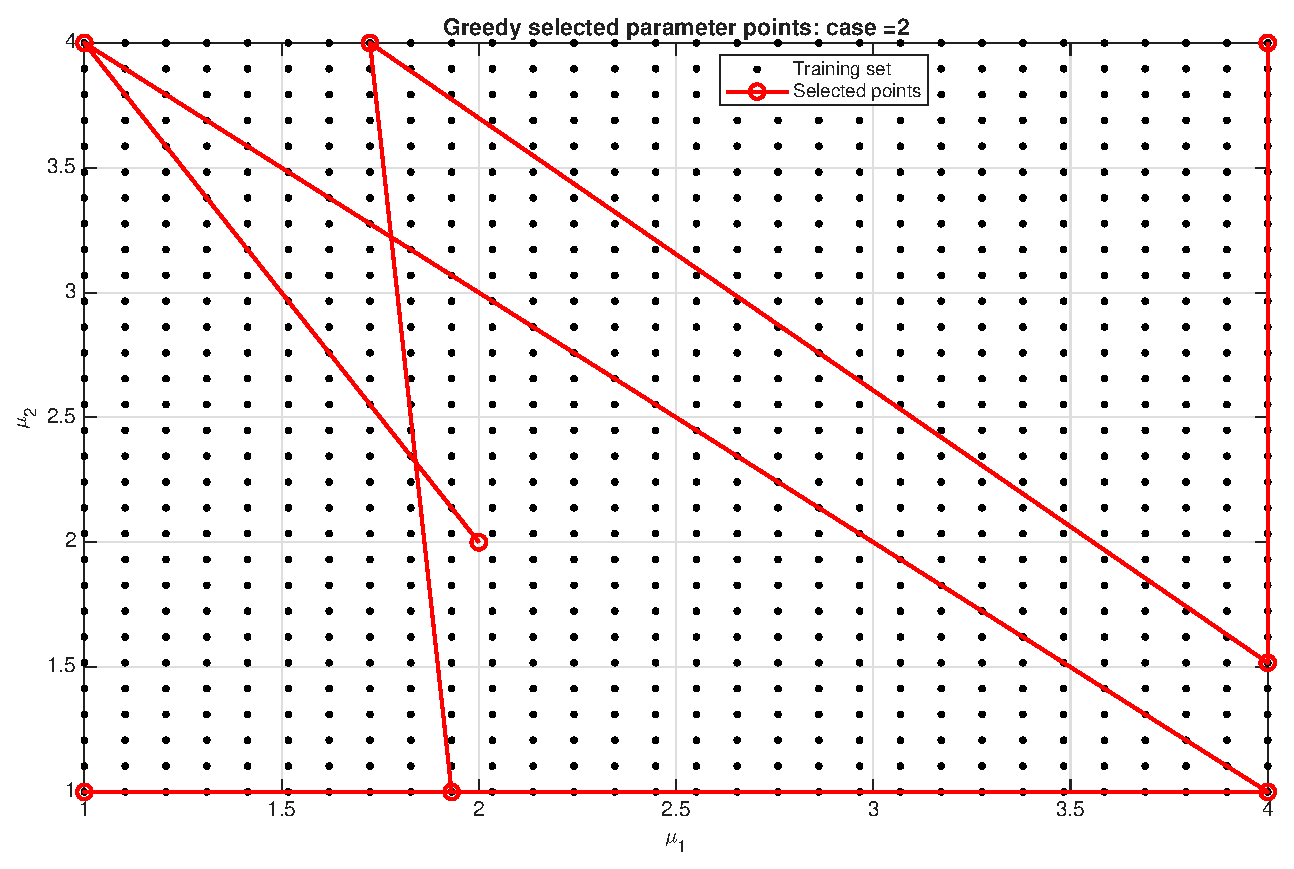
\includegraphics[width=0.5\textwidth]{img/GSP_case2_basis2_err2.eps}
	%	
\includegraphics[width=0.29\textwidth]{img/solplot_N80_k15_k29.eps}
	%	\caption{Graph of FEM and Exact solution When $x_k =0.5$ is a node}
	%	\label{fig:N1}
\end{figure}
\clearpage
\item[Case 3: ] RB space $V_m = \text{span}\{U_h(\mu_j), j =1,\ldots,m\}$, with $L_1$ error indicator
\begin{figure}[htbp]
	\centering
	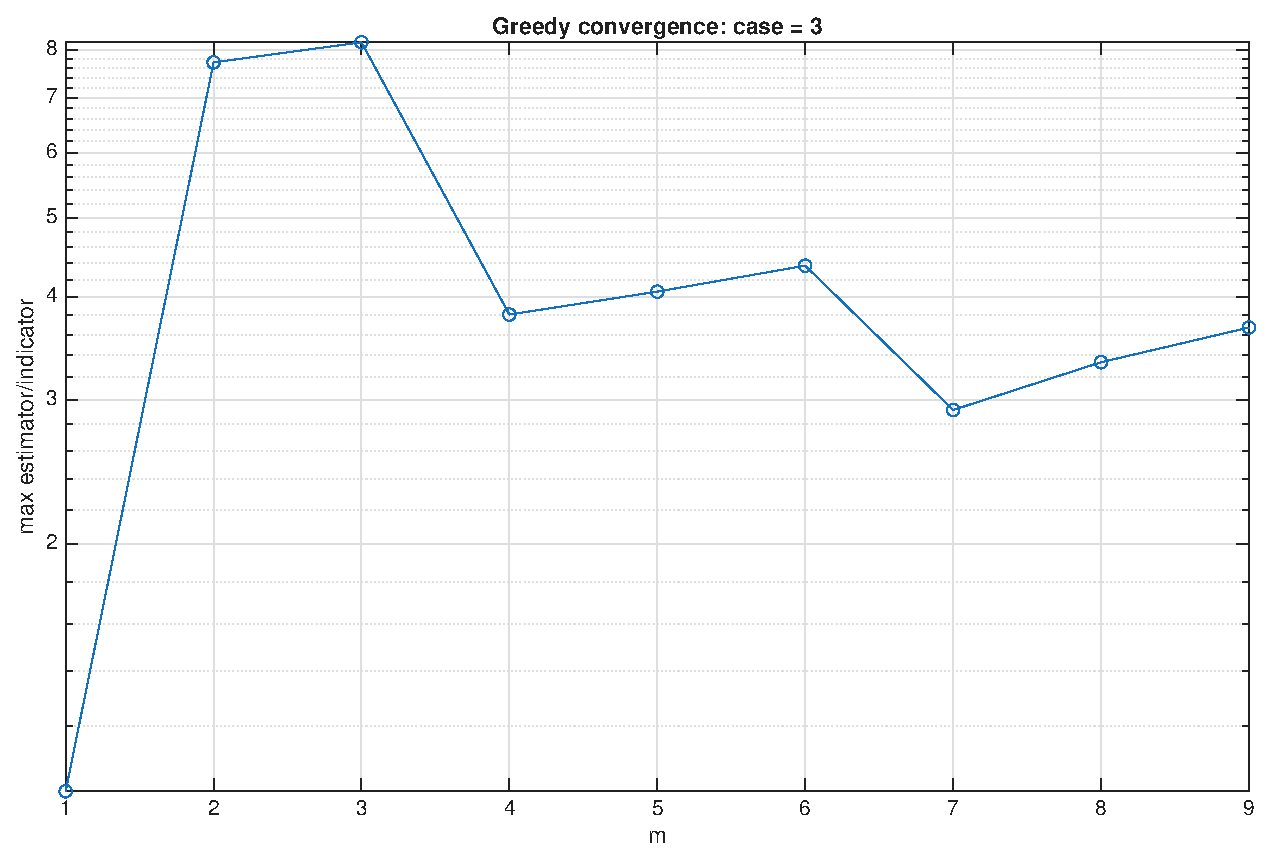
\includegraphics[width=0.5\textwidth]{img/GC_case3_basis1_err1.eps}
	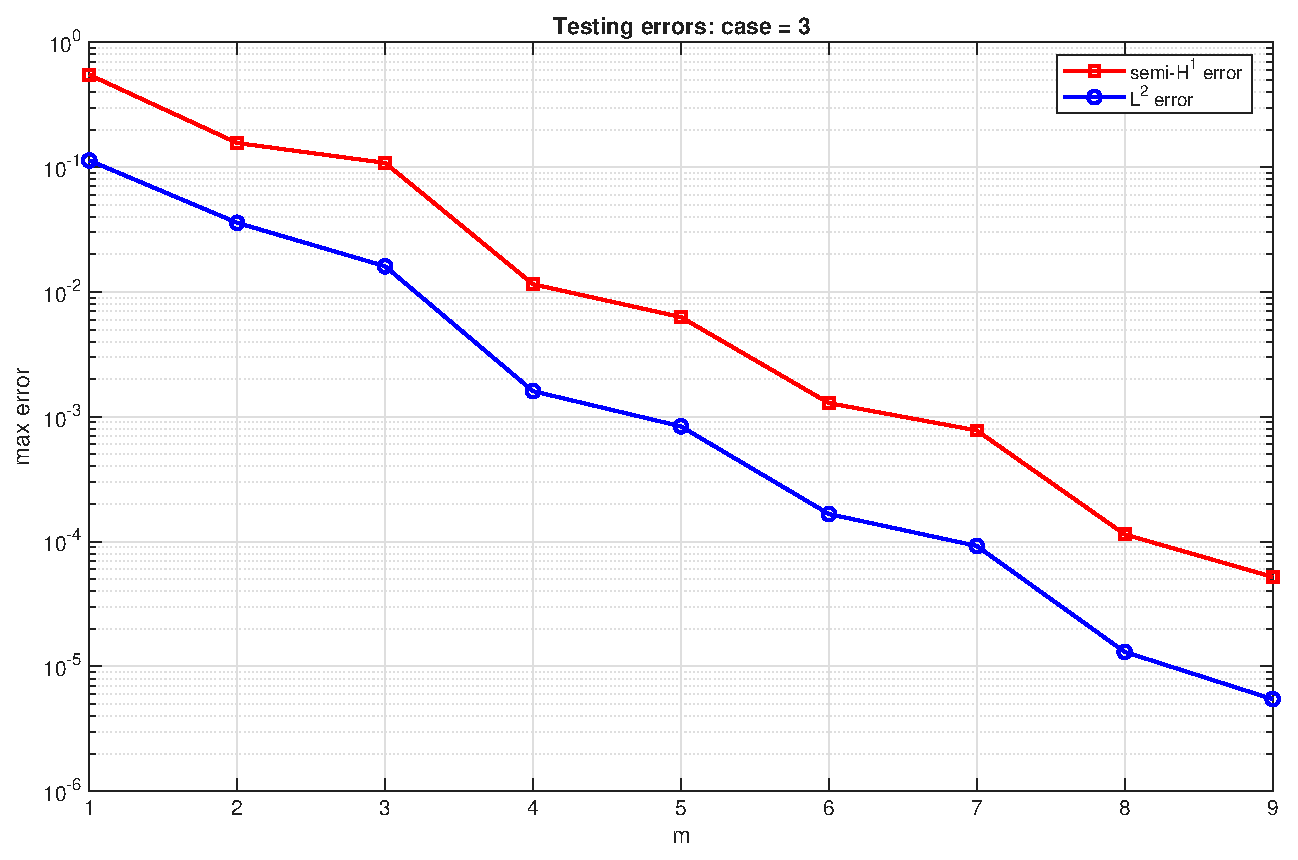
\includegraphics[width=0.5\textwidth]{img/TE_case3_basis1_err1.eps}
	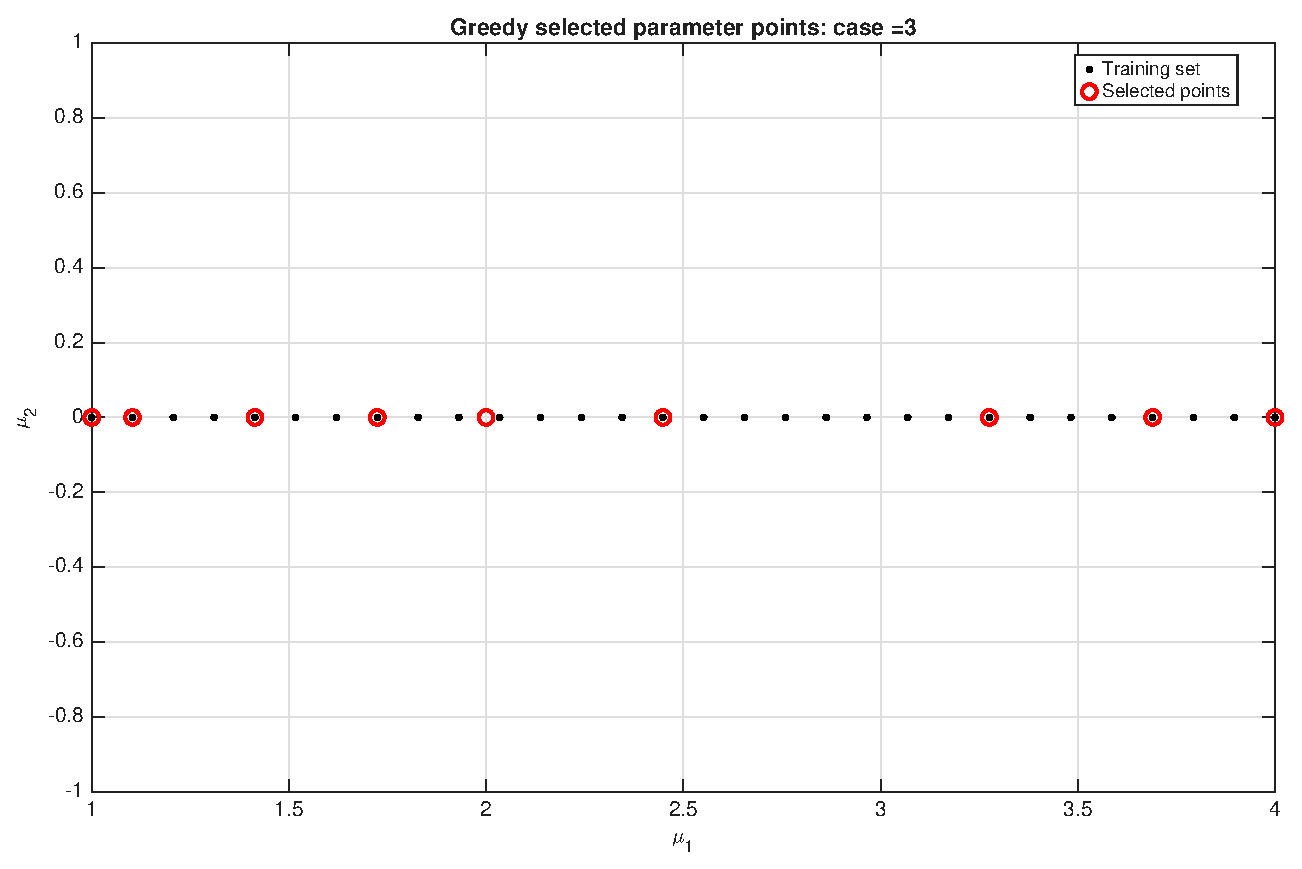
\includegraphics[width=0.5\textwidth]{img/GSP_case3_basis1_err1.eps}
	%	
\includegraphics[width=0.29\textwidth]{img/solplot_N80_k15_k29.eps}
	%	\caption{Graph of FEM and Exact solution When $x_k =0.5$ is a node}
	%	\label{fig:N1}
\end{figure}
\clearpage
\item[Case 3: ] RB space $V_m = \text{span}\{U_h(\mu_j), j =1,\ldots,m\}$, with residual error estimator
\begin{figure}[htbp]
	\centering
	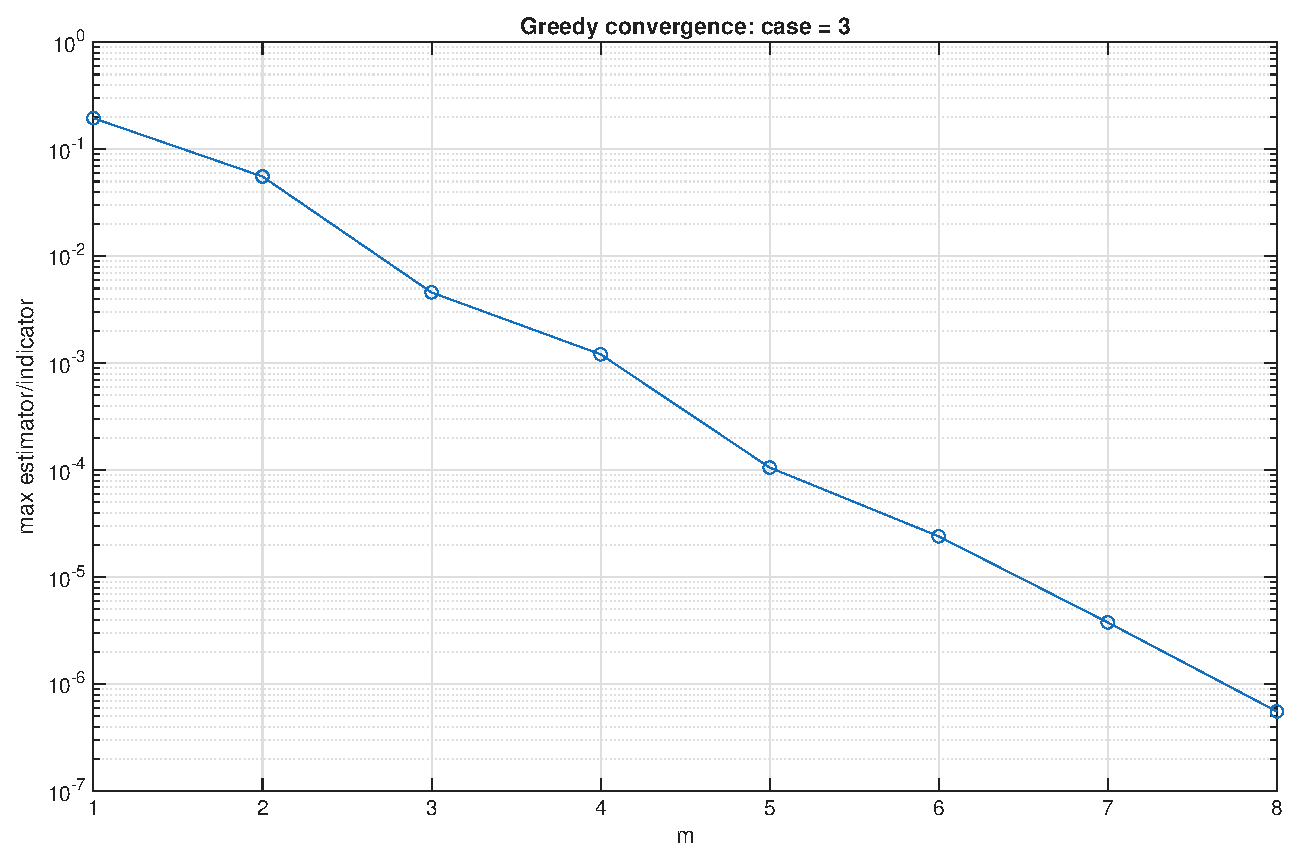
\includegraphics[width=0.5\textwidth]{img/GC_case3_basis1_err2.eps}
	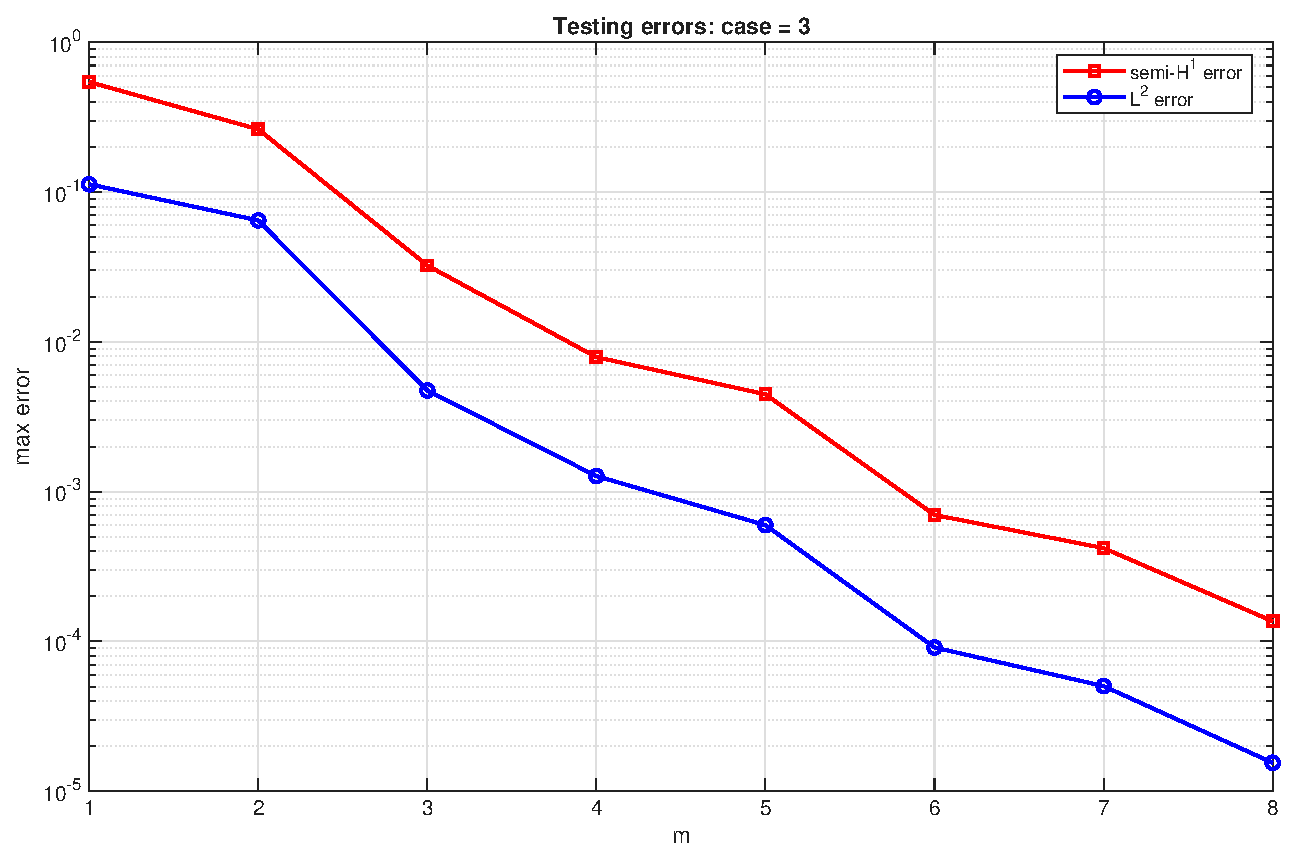
\includegraphics[width=0.5\textwidth]{img/TE_case3_basis1_err2.eps}
	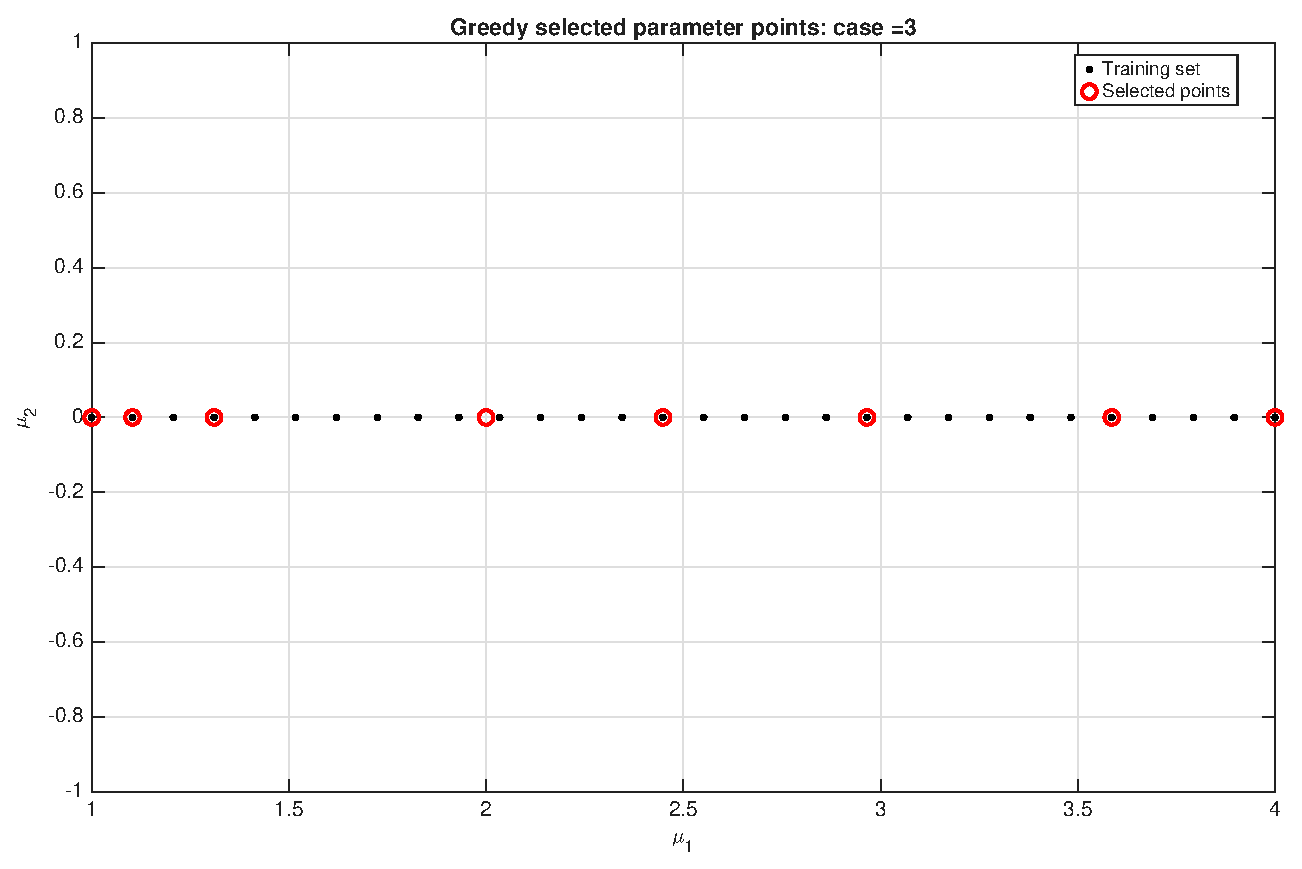
\includegraphics[width=0.5\textwidth]{img/GSP_case3_basis1_err2.eps}
	%	
\includegraphics[width=0.29\textwidth]{img/solplot_N80_k15_k29.eps}
	%	\caption{Graph of FEM and Exact solution When $x_k =0.5$ is a node}
	%	\label{fig:N1}
\end{figure}
\clearpage
\item[Case 3: ] QR factorization, with $L_1$ error indicator
\begin{figure}[htbp]
	\centering
	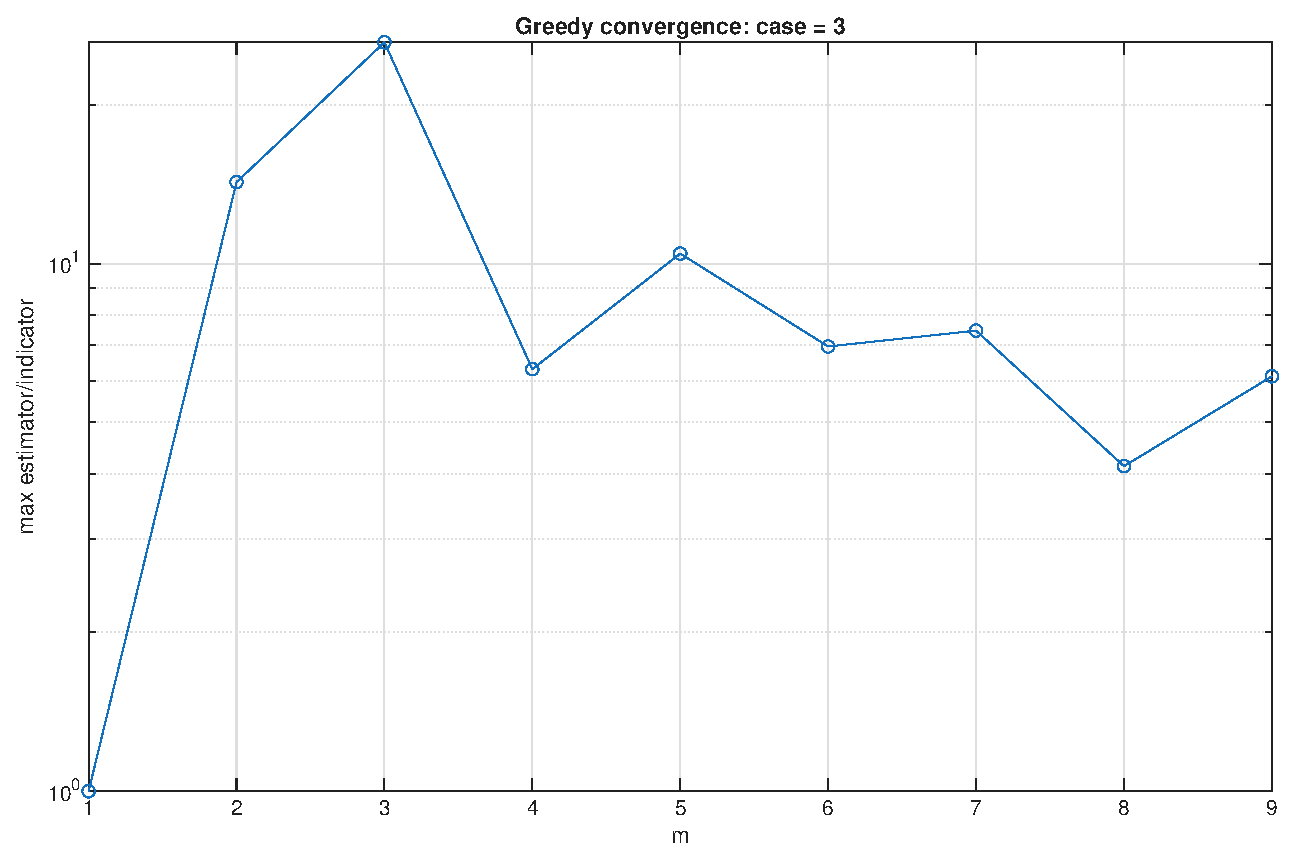
\includegraphics[width=0.5\textwidth]{img/GC_case3_basis2_err1.eps}
	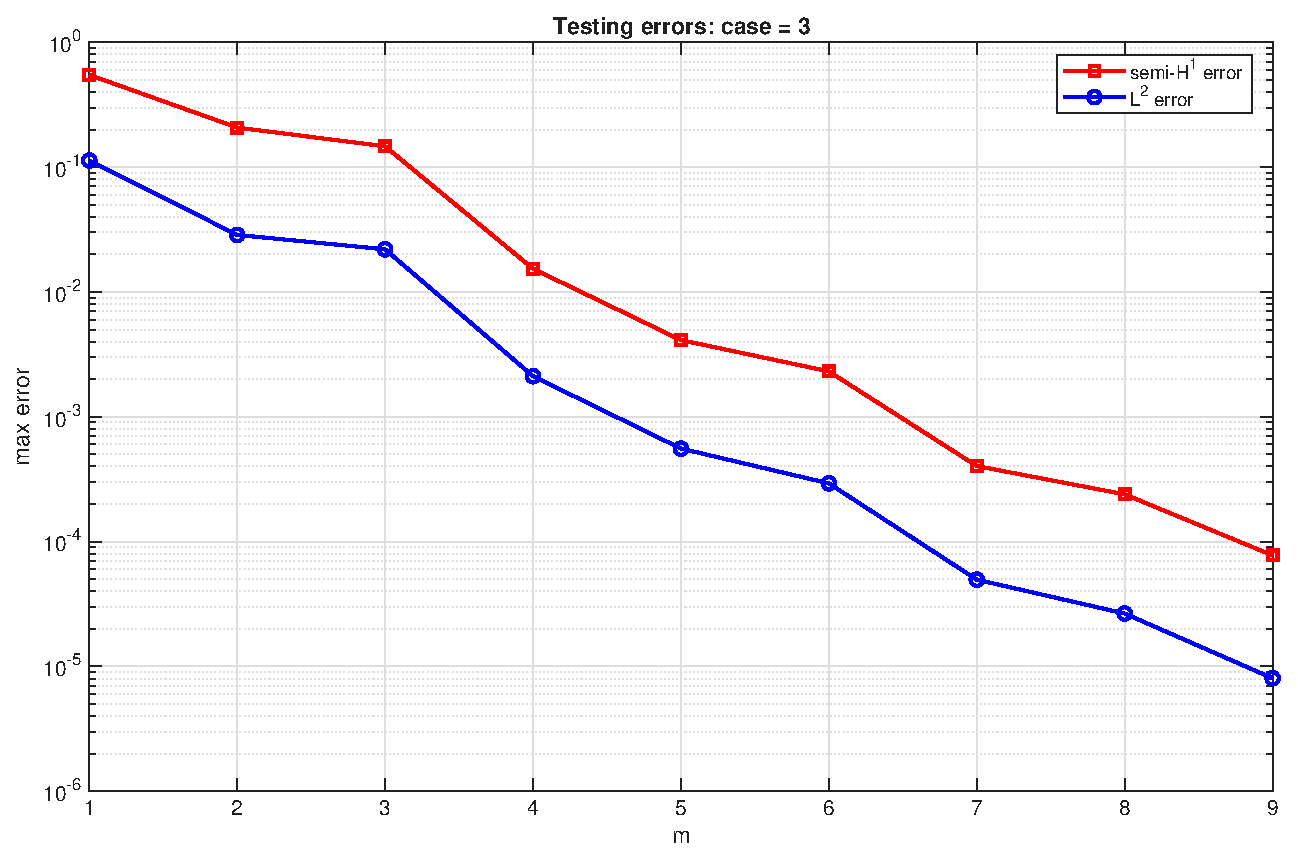
\includegraphics[width=0.5\textwidth]{img/TE_case3_basis2_err1.eps}
	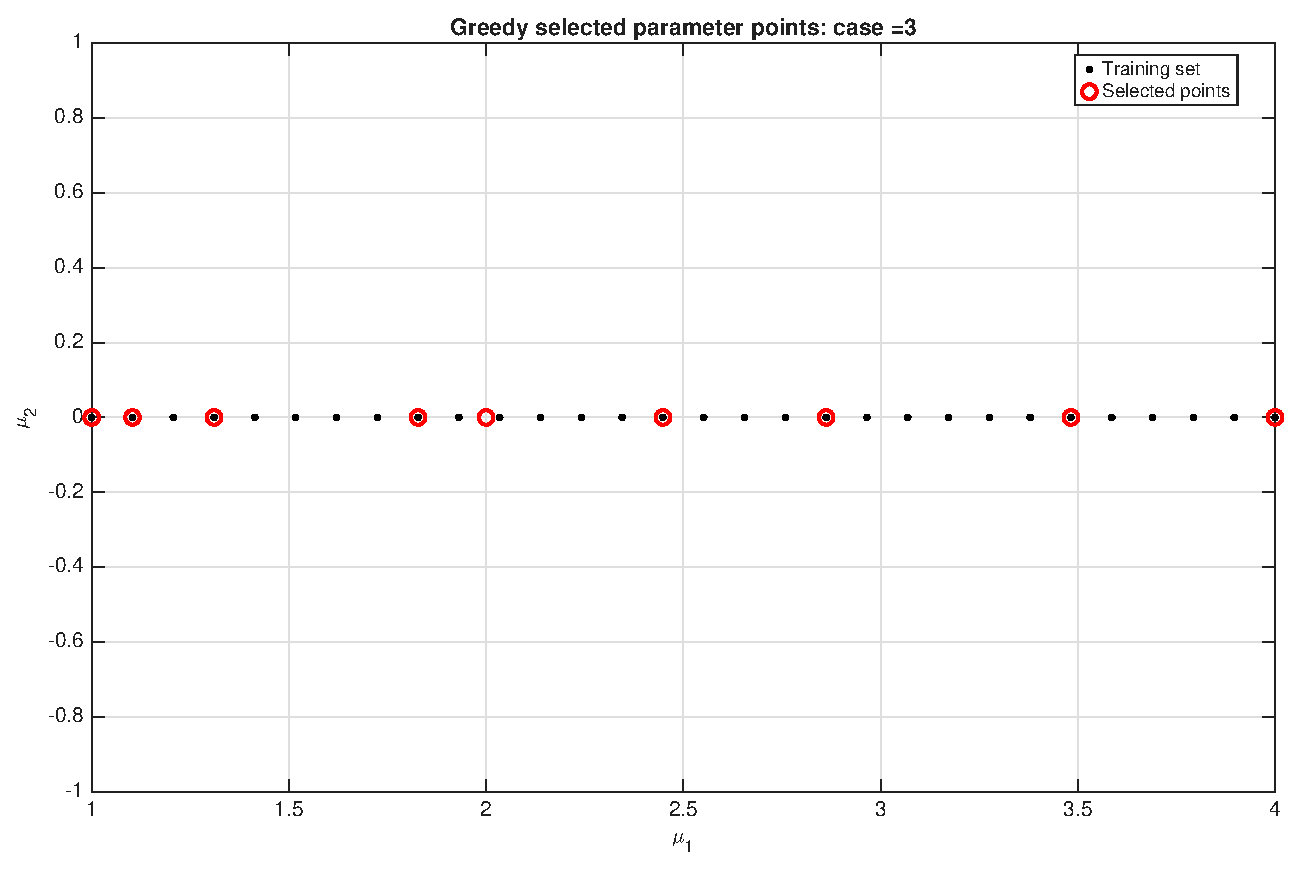
\includegraphics[width=0.5\textwidth]{img/GSP_case3_basis2_err1.eps}
	%	
\includegraphics[width=0.29\textwidth]{img/solplot_N80_k15_k29.eps}
	%	\caption{Graph of FEM and Exact solution When $x_k =0.5$ is a node}
	%	\label{fig:N1}
\end{figure}
\clearpage
\item[Case 3: ] QR factorization, with residual error estimator
\begin{figure}[htbp]
	\centering
	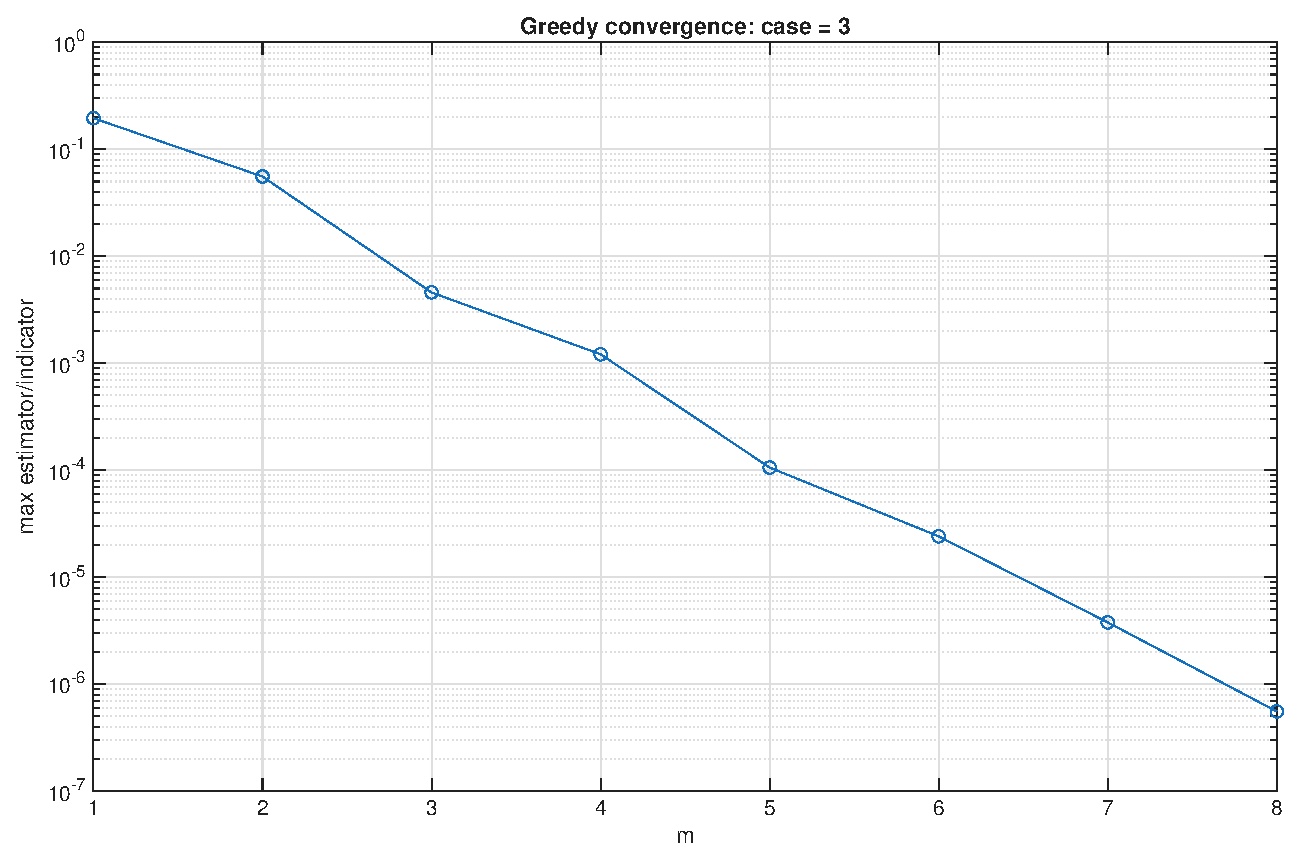
\includegraphics[width=0.5\textwidth]{img/GC_case3_basis2_err2.eps}
	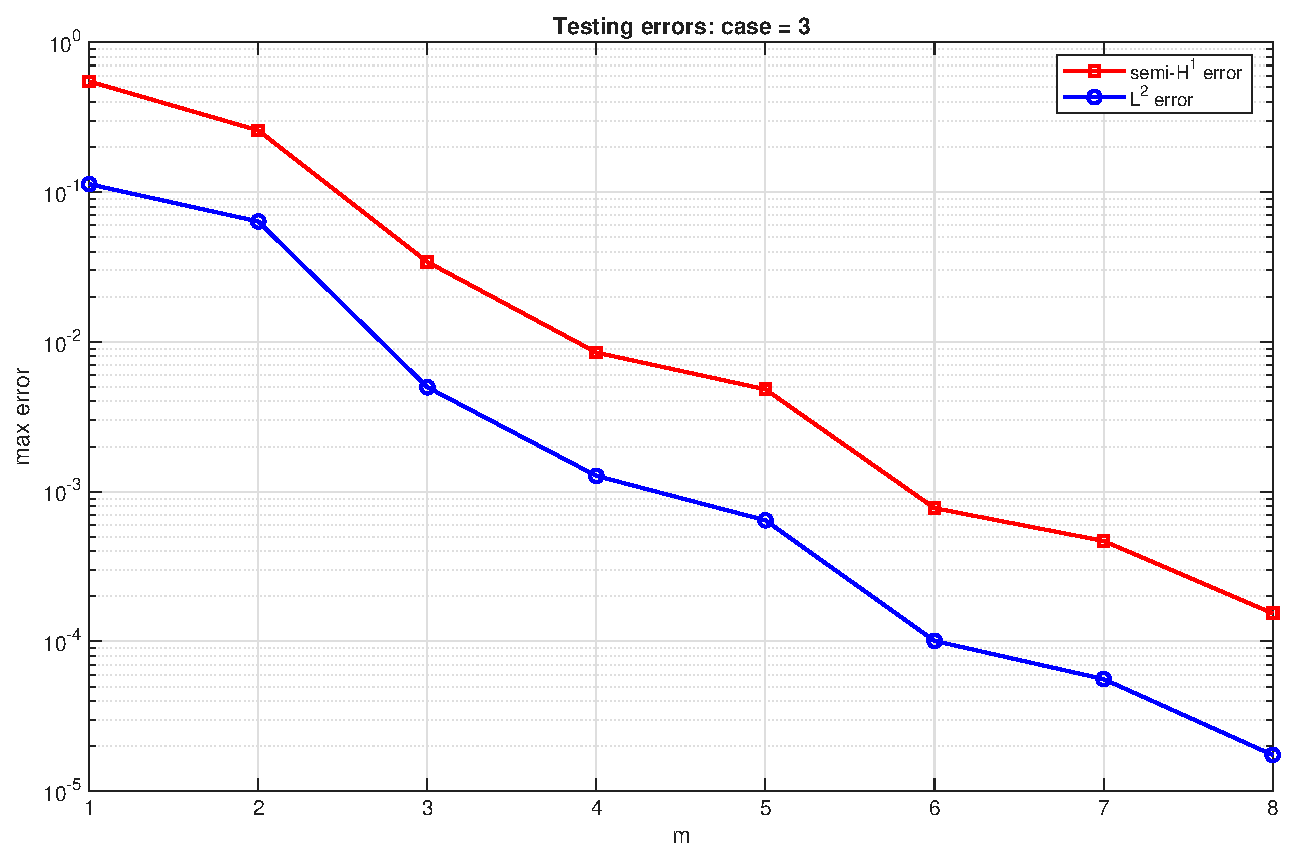
\includegraphics[width=0.5\textwidth]{img/TE_case3_basis2_err2.eps}
	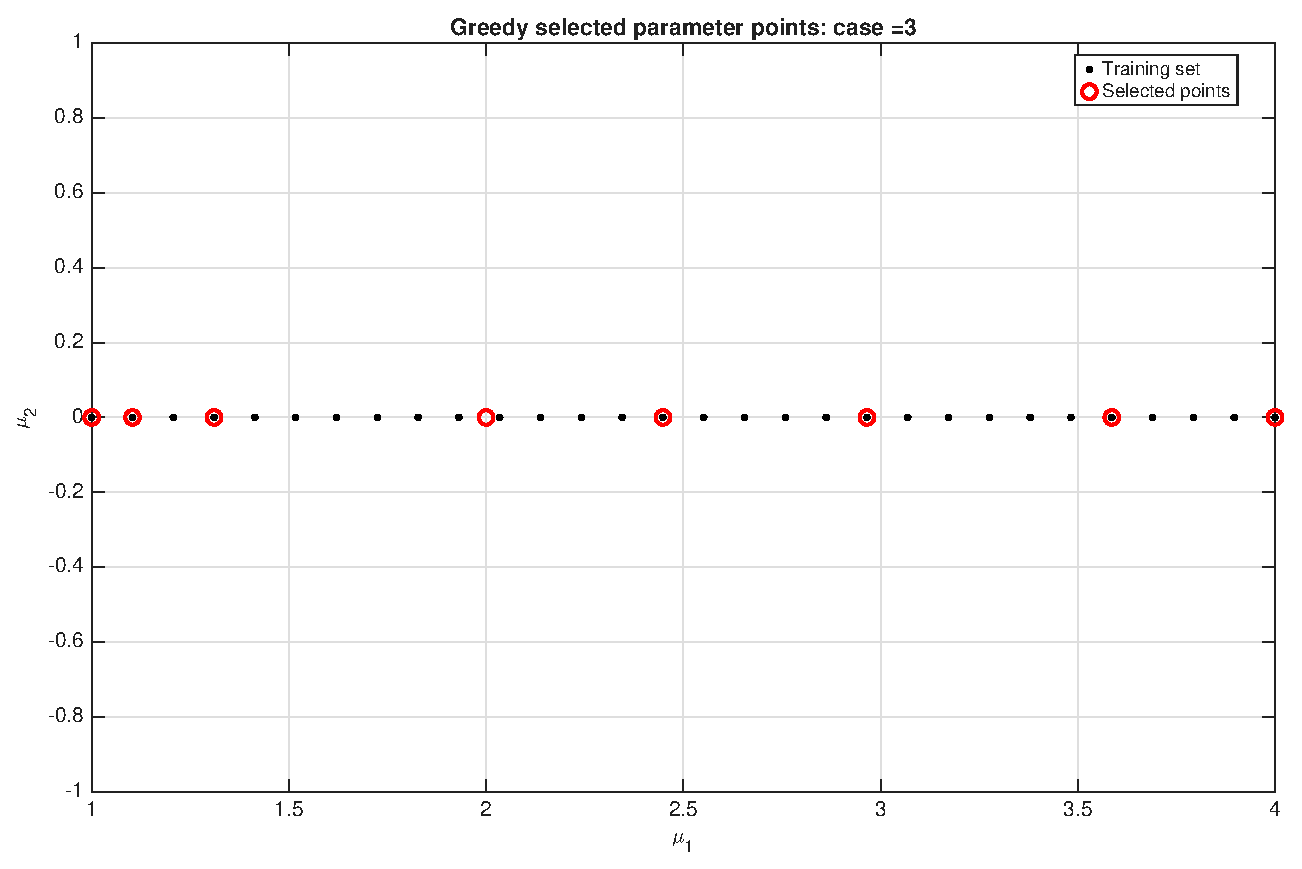
\includegraphics[width=0.5\textwidth]{img/GSP_case3_basis2_err2.eps}
	%	
\includegraphics[width=0.29\textwidth]{img/solplot_N80_k15_k29.eps}
	%	\caption{Graph of FEM and Exact solution When $x_k =0.5$ is a node}
	%	\label{fig:N1}
\end{figure}
\section*{conclusion}
The Reduced Basis Method (RBM) was tested using the finite element method (FEM) solution as the high-fidelity reference across three different parameterized cases. For each case, four configurations were considered:
\begin{itemize}
	\item Standard RB space with $\ell_1$-indicator,
	\item Standard RB space with residual-based estimator,
	\item QR-orthonormalized basis with $\ell_1$-indicator,
	\item QR-orthonormalized basis with residual-based estimator.
\end{itemize}
Across all cases, the greedy algorithm exhibits a monotonic decay of testing errors. The greedy algorithm selects parameter points that are well distributed over the parameter domain. The selected points tend to concentrate in regions where the solution exhibits stronger variation, demonstrating the adaptive nature of the method.
The residual-based estimator shows faster and more stable convergence, typically reaching the prescribed tolerance with fewer basis functions (approximately $m \approx 8$). In contrast, the $\ell_1$-based indicator converges more slowly and may require a larger reduced basis dimension to achieve comparable accuracy. I set the maximum dimension of the reduced basis to 9. That's why the $m*=9$ for $\ell_1$ error indicator. The plot for the greedy convergence for $\ell_1$ error indicator does not tell us much about how the testing errors, rather it helpd to select the next parameter to use in building the RB basis.

The semi-$H_1$ and $L_2$ errors decrease rapidly as the reduced basis dimension increases. The decay is approximately exponential.
The residual-based greedy approach consistently yields lower errors for a given basis size. The use of QR factorization improves numerical stability and conditioning of the reduced system, although it does not significantly affect the convergence rate.

Overall, the RBM significantly reduces computational cost while maintaining high accuracy, making it well-suited for repeated evaluations in parametrized problems.
\end{enumerate}
\lstinputlisting[language=matlab, numbers=left, stepnumber=1, firstline=1,caption={main.m },label=code:main,frame=single]{main.m}
\lstinputlisting[language=matlab, numbers=left, stepnumber=1, firstline=1,caption={solveFEM.m },label=code:Meshgen,frame=single]{solveFEM.m}
\lstinputlisting[language=matlab, numbers=left, stepnumber=1, firstline=1,caption={solveROM.m },label=code:main2,frame=single]{solveROM.m}
\lstinputlisting[language=matlab, numbers=left, stepnumber=1, firstline=1,caption={MatrixCase1.m },label=code:main3,frame=single]{MatrixCase1.m}
\lstinputlisting[language=matlab, numbers=left, stepnumber=1, firstline=1,caption={MatrixCase2.m },label=code:main4,frame=single]{MatrixCase2.m}
\lstinputlisting[language=matlab, numbers=left, stepnumber=1, firstline=1,caption={MatrixCase3.m },label=code:main5,frame=single]{MatrixCase3.m}
%\lstinputlisting[language=matlab, numbers=left, stepnumber=1, firstline=1,caption={$U_h (x,y)$ function },label=code:main4,frame=single]{UhElement.m}
%\lstinputlisting[language=matlab, numbers=left, stepnumber=1, firstline=1,caption={$e_h(x,y)$ function },label=code:main5,frame=single]{getErrors.m}
%\lstinputlisting[language=matlab, numbers=left, stepnumber=1, firstline=1,caption={main.m },label=code:main1D,frame=single]{1D problem/main.m}
%\lstinputlisting[language=matlab, numbers=left, stepnumber=1, firstline=1,caption={twoPointBVP.m },label=code:twoP1D,frame=single]{1D problem/twoPointBVP.m}
%\lstinputlisting[language=matlab, numbers=left, stepnumber=1, firstline=1,caption={formMatrix.m },label=code:main31,frame=single]{1D problem/formMatrix.m}
%\lstinputlisting[language=matlab, numbers=left, stepnumber=1, firstline=1,caption={$U_h (x)$ function },label=code:main41,frame=single]{1D problem/UhFunc.m}
%\lstinputlisting[language=matlab, numbers=left, stepnumber=1, firstline=1,caption={$U_{hx}(x)$ function },label=code:main51,frame=single]{1D problem/UhFuncx.m}
\end{document}               % End of document.
